% This LaTeX document needs to be compiled with XeLaTeX.
\documentclass[10pt]{article}
\usepackage[utf8]{inputenc}
\usepackage{graphicx}
\usepackage[export]{adjustbox}
\graphicspath{ {./images/} }
\usepackage{amsmath}
\usepackage{amsfonts}
\usepackage{amssymb}
\usepackage[version=4]{mhchem}
\usepackage{stmaryrd}
\usepackage[fallback]{xeCJK}
\usepackage{polyglossia}
\usepackage{fontspec}
\setCJKmainfont{Noto Serif CJK SC}

\setmainlanguage{french}
\setmainfont{CMU Serif}

\title{ÉCOLE DES PONTS PARISTECH, ISAE-SUPAERO, ENSTA PARIS, TELECOM PARIS, MINES PARISTECH, MINES SAINT-ÉTIENNE, MINES NANCY, IMT Atlantique, ENSAE PARIS, CHIMIE PARISTECH - PSL. }

\author{}
\date{}


%New command to display footnote whose markers will always be hidden
\let\svthefootnote\thefootnote
\newcommand\blfootnotetext[1]{%
  \let\thefootnote\relax\footnote{#1}%
  \addtocounter{footnote}{-1}%
  \let\thefootnote\svthefootnote%
}

%Overriding the \footnotetext command to hide the marker if its value is `0`
\let\svfootnotetext\footnotetext
\renewcommand\footnotetext[2][?]{%
  \if\relax#1\relax%
    \ifnum\value{footnote}=0\blfootnotetext{#2}\else\svfootnotetext{#2}\fi%
  \else%
    \if?#1\ifnum\value{footnote}=0\blfootnotetext{#2}\else\svfootnotetext{#2}\fi%
    \else\svfootnotetext[#1]{#2}\fi%
  \fi
}

\begin{document}
\maketitle
Concours Mines-Télécom, Concours Centrale-Supélec (Cycle International).

CONCOURS 2023

\section*{ÉPREUVE DE SCIENCES INDUSTRIELLES}
\section*{Durée de l'épreuve : 4 heures}
L'usage de la calculatrice ou de tout dispositif électronique est interdit.

L'énoncé de cette épreuve comporte 13 pages de texte et un complément de 5 pages regroupant les annexes de 1 à 5 .

Le travail doit être reporté sur un document-réponse de 16 pages distribué avec le sujet. Un seul document-réponse est fourni au candidat.

Le renouvellement de ce document en cours d'épreuve est interdit.

Pour valider ce document-réponse, chaque candidat doit obligatoirement y inscrire à l'encre, à l'intérieur du rectangle d'anonymat situé en haut de chaque copie, ses nom, prénoms, numéro d'inscription et signature.

Si, au cours de l'épreuve, un candidat repère ce qui lui semble être une erreur d'énoncé,

il le signale sur sa copie et poursuit sa composition en expliquant les raisons des initiatives qu'il est amené à prendre.
\footnotetext{Les sujets sont la propriété du GIP CCMP. Ils sont publiés selon les termes de la licence Creative Commons Attribution - Pas d'Utilisation Commerciale - Pas de Modification 3.0 France. Tout autre usage est soumis à une autorisation préalable du Concours commun Mines Ponts.
}

\section*{ÉTUDE DU SISMOMÈTRE SEIS}
\section*{1 Présentation}
Après des années de recherche et de développement puis un voyage de 485 millions de kilomètres, la sonde InSight (Interior Exploration using Seismic Investigations, Geodesy and Heat Transport) s'est posée sur Mars le 26 novembre 2018. Elle est le premier observatoire géophysique martien, dont l'objectif est d'étudier la structure interne de Mars et de comprendre la formation et l'évolution des planètes rocheuses du Système solaire. En mesurant la façon dont les ondes sismiques, provoquées par des séismes martiens ou des impacts de météorites, se propagent à l'intérieur de Mars, les géophysiciens vont pouvoir répondre avec précision à cet objectif.

\begin{center}
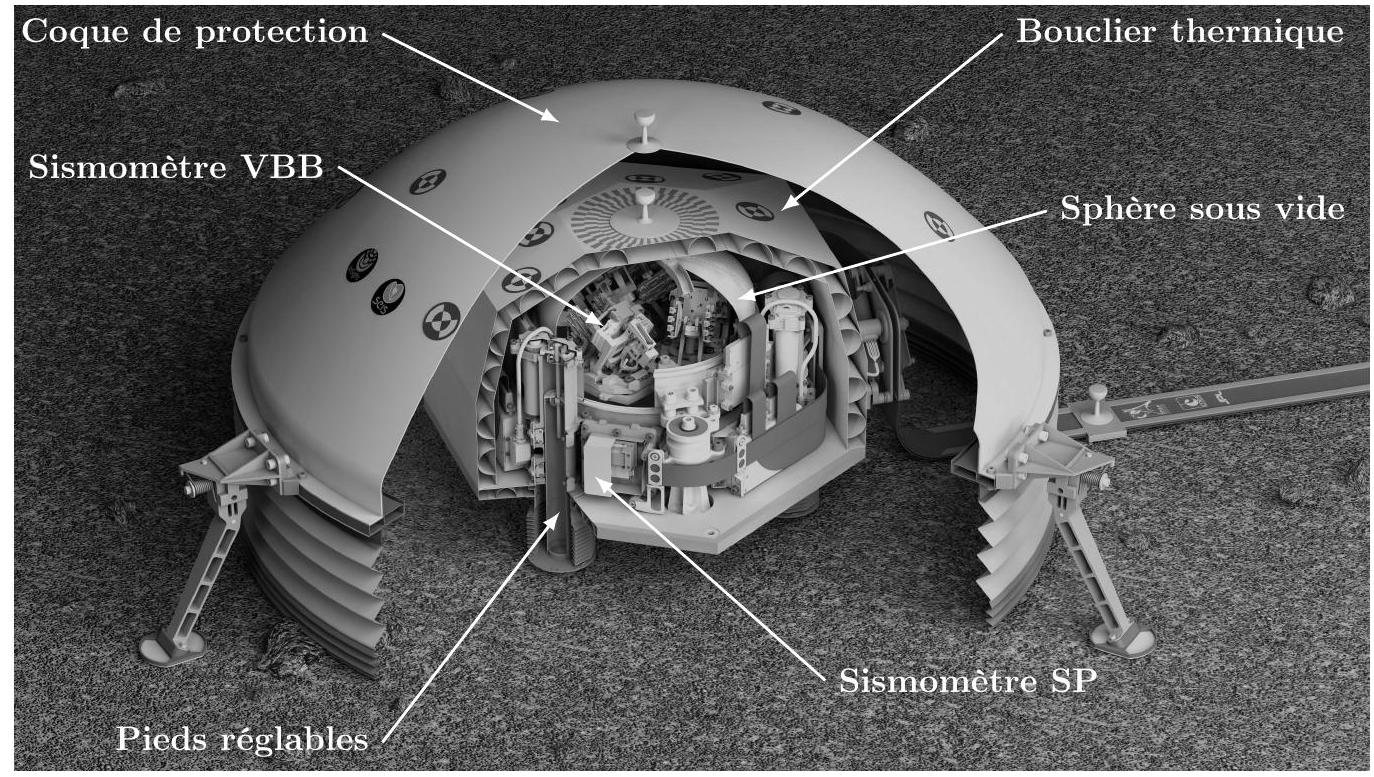
\includegraphics[max width=\textwidth]{2024_04_26_3285cfc264024262add0g-02}
\end{center}

FigURE 1 - Écorché de SEIS et ses différents niveaux de protection

Le sismomètre SEIS (Seismic Experiment for Interior Structures), déployé à la surface de Mars, est protégé des variations de la température et du vent à l'aide d'un bouclier thermique et d'une coque de protection. SEIS comporte deux sismomètres indépendants, le VBB (Very Broad Band) et le SP (Short Periods), montés sur une structure commune pouvant être réglée à l'horizontale grâce à des pieds de longueur variable.

\begin{itemize}
  \item Le sismomètre VBB comporte trois systèmes identiques, composés chacun d'un pendule et d'un bâti, inclinés différemment par rapport au sol. Ils sont fixés dans une sphère en titane sous vide, et sensibles à une large bande de fréquence d'ondes sismiques, entre 0,01 Hz et $0,5 \mathrm{~Hz}$.
  \item Le sismomètre SP est adapté aux ondes sismiques de plus hautes fréquences, entre 0,1 et $50 \mathrm{~Hz}$.
\end{itemize}

\begin{center}
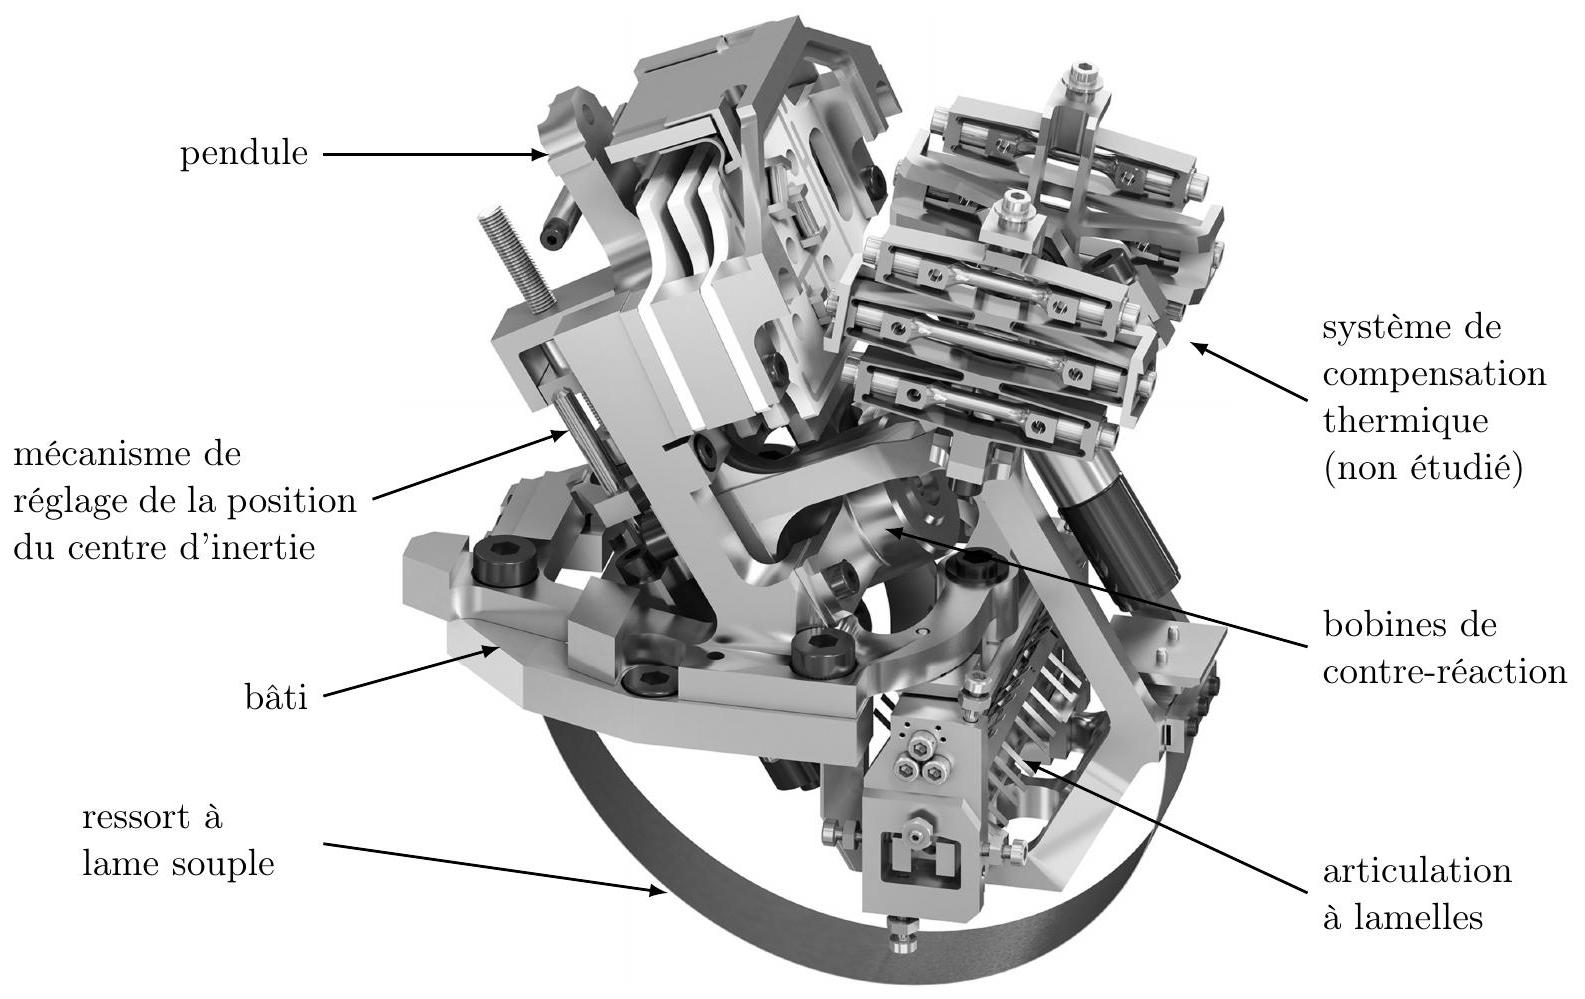
\includegraphics[max width=\textwidth]{2024_04_26_3285cfc264024262add0g-03}
\end{center}

Figure 2 - Vue 3D d'un des trois systèmes du VBB

Dans ce sujet, on s'attache à valider certaines étapes clés de la conception et du réglage d'un des trois systèmes du sismomètre VBB. Cette dernière étape ayant eu lieu sur Terre, il a fallu contourner les difficultés liées aux différences de gravité et de température entre la Terre et Mars.

Une vue détaillée d'un des systèmes du VBB est fournie en FiguRe 2 et le détail des différents éléments qui le constituent est fourni en Annexe 1.

\section*{2 Réglage de la position d'équilibre du pendule}
Comme pour les applications terrestres, chaque système du sismomètre VBB possède un pendule qui oscille par rapport à un bâti sous l'impulsion de secousses sismiques transmises par le sol à l'instrument. Une articulation à lamelles permet des mouvements de très faible amplitude avec un minimum de frottements visqueux entre le pendule et le bâti, et sans jeu. Elle constitue l'axe de rotation du pendule dans son mouvement par rapport au bâti.

Le sismomètre VBB s'appuie sur le principe du pendule inversé. L'instabilité inhérente au pendule inversé lui confère une plus grande sensibilité que celle d'un pendule classique. Bien qu'instable par nature, le pendule inversé du sismomètre VBB conserve son équilibre grâce à un ressort à lame souple, recourbé en demi-cercle, et qui applique en permanence une action mécanique de rappel.

\subsection*{2.1 Compensation de la gravité terrestre}
Le sismomètre étant optimisé pour fonctionner sous gravité martienne, il n'est pas possible de le tester sur Terre sans y apporter des modifications. En effet, pour un mouvement du sol donné sur Terre, l'amplitude résultante des oscillations du pendule risquerait de détériorer le mécanisme. Un contrepoids est ajouté au pendule, dont le moment généré sur son axe de rotation par rapport au bâti doit compenser celui dû à la différence de gravité entre la Terre et Mars (voir FigURe 3b).

\begin{center}
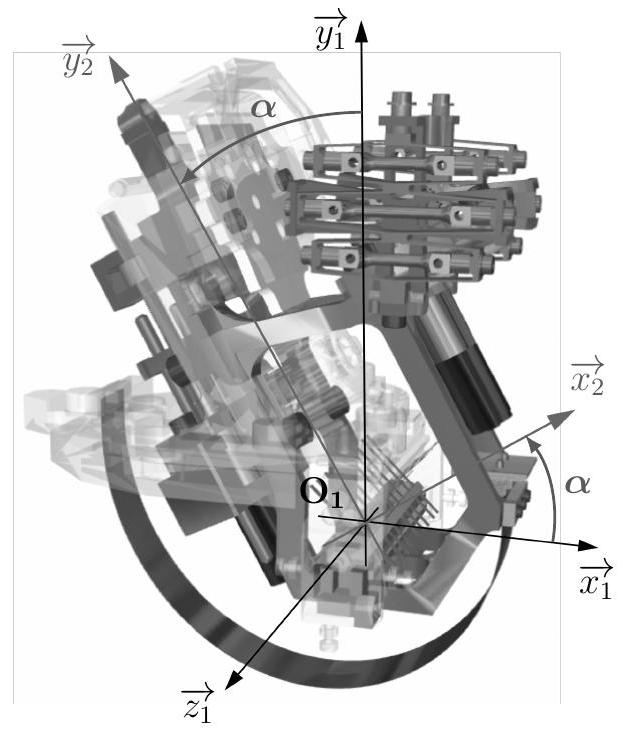
\includegraphics[max width=\textwidth]{2024_04_26_3285cfc264024262add0g-04}
\end{center}

(a) Pendule en niveaux de gris; bâti en transparence (voir aussi Annexe 1).

\begin{center}
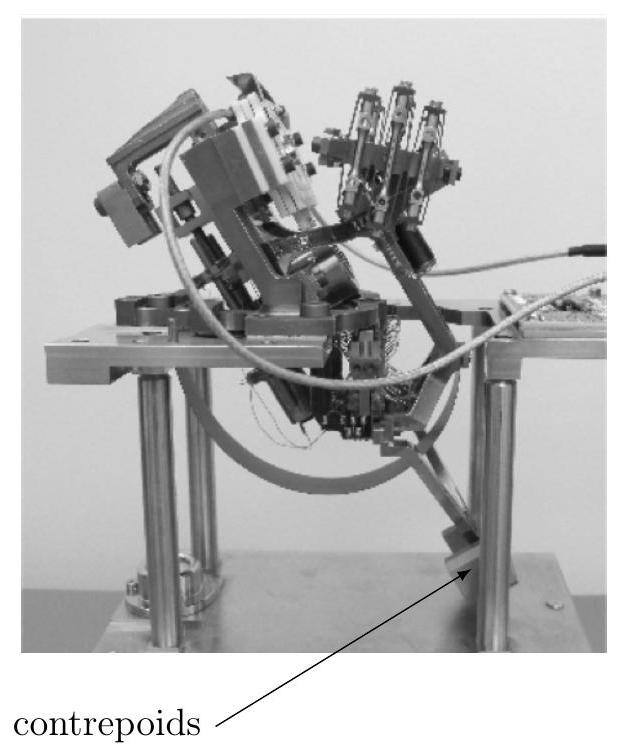
\includegraphics[max width=\textwidth]{2024_04_26_3285cfc264024262add0g-04(1)}
\end{center}

(b) Dispositif expérimental avec contrepoids pour tester les oscillations du pendule sur Terre

FIGURE 3

Objectif : établir les conditions que doit respecter le contrepoids pour compenser la gravité terrestre lors d'expériences sur Terre.

Le schéma cinématique et le paramétrage du dispositif sont fournis en Annexe 2, ainsi que l'ensemble des notations et hypothèses utiles pour cette sous-partie.

On désigne par «ensemble mobile»le pendule noté (2) équipé du contrepoids noté (3). Le bâti, lié au sol, est noté (1).

Q1. Écrire l'équation traduisant l'équilibre de l'ensemble mobile $\{(2)+(3)\}$ sur Terre, lorsque $\alpha(t)=\alpha_{\mathrm{eq}}$. Préciser le bilan des actions mécaniques extérieures, le théorème ou principe utilisé, et les éléments d'application (projection, point éventuel).

Sur Mars, le pendule (2) n'est pas équipé du contrepoids (3). Cependant, la position d'équilibre du pendule (2) sans contrepoids (3) sur Mars, et celle du pendule (2) avec le contrepoids (3) sur Terre, doivent être identiques.

Q2. Donner la condition sur la masse $m_{3}$ et la variable $b$ pour compenser la différence de pesanteur entre la Terre et Mars. Pour cela, exprimer le produit $b m_{3}$ en fonction de $a$, $M_{2}, g_{T}$ et $g_{M}$.

Cette condition étant respectée, on peut alors traduire l'équilibre de l'ensemble mobile sur Terre :


\begin{equation*}
a M_{2} g_{\mathrm{M}} \sin \alpha_{\mathrm{eq}}+C_{0}-k\left(\alpha_{\mathrm{eq}}-\alpha_{0}\right)=0 \tag{eq.1}
\end{equation*}


\subsection*{2.2 Conception d'un mécanisme de translation du centre d'inertie du pendule}
Si l'inclinaison de la surface sur laquelle le sismomètre est posé n'est pas correctement corrigée par les pieds réglables, la position $a$ du centre d'inertie $G_{2}$ du pendule (2) le long de l'axe $\left(O_{1}, \overrightarrow{y_{2}}\right)$ peut être réglée à distance. Cela permet notamment d'assurer que $\alpha_{\mathrm{eq}}$ conserve une valeur optimale déterminée lors d'expérimentations sur Terre.

Pour cela, un mécanisme embarqué sur (2), constitué d'un moteur pas-à-pas, d'un réducteur à train épicycloïdal, d'un joint d'accouplement (joint d'Oldham) et d'un système vis-écrou, indiqués en Figure 4, est guidé en translation le long de l'axe ( $\left.O_{1}, \overrightarrow{y_{2}}\right)$.

Objectif : justifier les choix de conception du mécanisme de translation du centre d'inertie du pendule.

\begin{center}
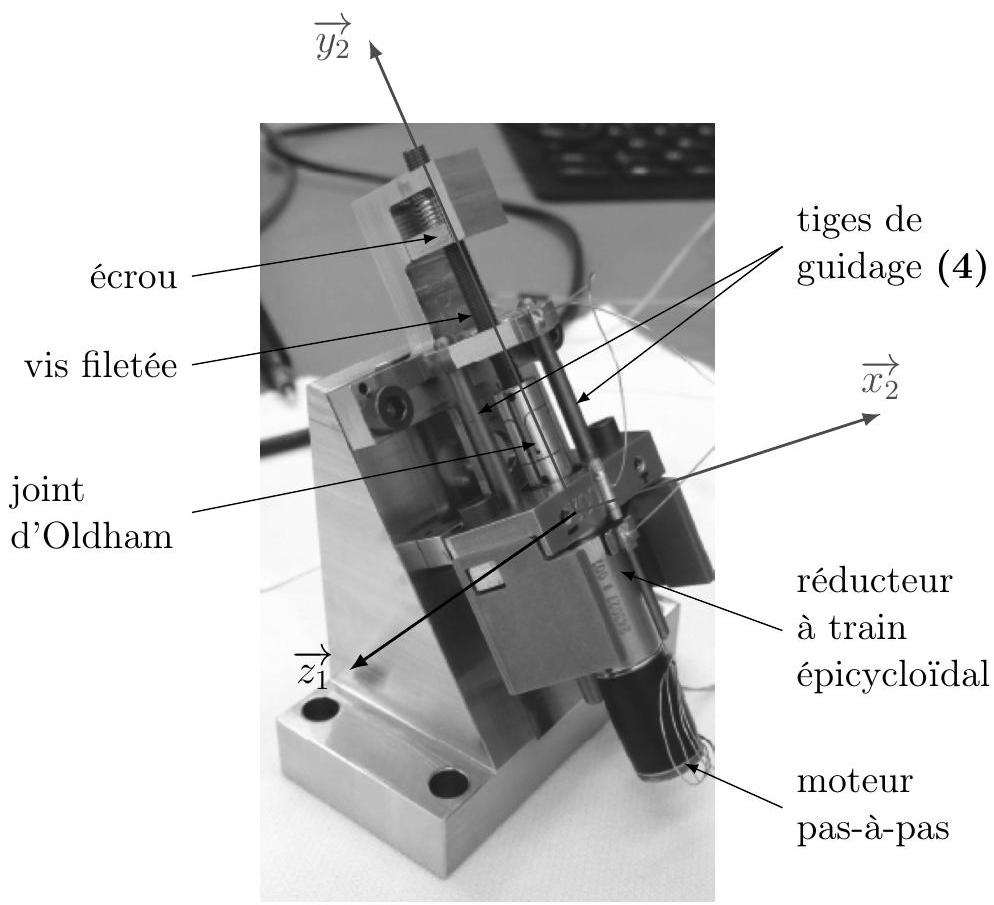
\includegraphics[max width=\textwidth]{2024_04_26_3285cfc264024262add0g-05(1)}
\end{center}

FiguRe 4 - Photographie du mécanisme de réglage de la position du centre d'inertie du pendule. Le mécanisme est ici fixé sur un support métallique incliné représentant le corps du pendule (2).

\begin{center}
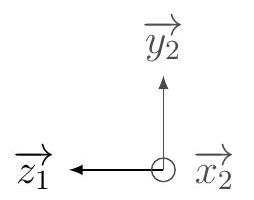
\includegraphics[max width=\textwidth]{2024_04_26_3285cfc264024262add0g-05(2)}
\end{center}

$(4)$

\begin{center}
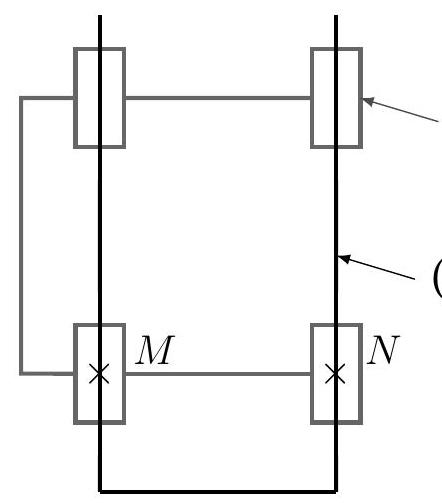
\includegraphics[max width=\textwidth]{2024_04_26_3285cfc264024262add0g-05}
\end{center}

Figure 5 - Schéma cinématique du guidage en translation des tiges (4) par rapport au corps du pendule (2)

Pendant la phase de réglage de la position de son centre d'inertie, on suppose que le corps du pendule (2) reste immobile. L'ensemble du mécanisme embarqué est considéré comme mobile par rapport au corps du pendule (2) le temps de cette étude.

Le guidage en translation des tiges (4) par rapport à (2) permettant le réglage de la position du centre d'inertie est réalisé par l'association de 4 liaisons en parallèle (voir FIGURE 5).

Q3. Compléter, sur le Cahier Réponses, le graphe des liaisons fourni avec les noms et la (les) caractéristique(s) géométrique(s) des liaisons. Donner le nombre de boucles indépendantes (nombre cyclomatique $\gamma$ ) de ce modèle.

Q4. Déterminer le degré d'hyperstatisme $h$ de ce modèle. Préciser les mobilités internes $\left(m_{i}\right)$ et utiles $\left(m_{u}\right)$. Justifier, au regard du système et de son contexte d'utilisation, l'intérêt d'un tel degré d'hyperstatisme pour la réalisation du guidage.

L'association des 4 liaisons en parallèle entre (4) et (2) correspond à une liaison glissière équivalente de direction $\overrightarrow{y_{2}}$. La suite de l'étude s'appuiera sur le schéma cinématique réduit de la FigURE 6 faisant apparaître cette liaison équivalente, ainsi que des éléments du mécanisme embarqué. Le schéma cinématique réduit de l'ensemble du mécanisme est fourni en Annexe 3.

Le joint de type Oldham assure l'accouplement de l'arbre (5) en sortie du réducteur à train épicycloïdal avec la vis (v).

La Figure 7 présente les éléments constitutifs d'un joint d'Oldham :

\begin{itemize}
  \item le plateau d'entrée est cinématiquement lié à l'arbre (5) en sortie du réducteur;
  \item le plateau de sortie est cinématiquement lié à la vis (v);
  \item la noix, repérée $(\mathbf{N})$, est la pièce intermédiaire du joint.
\end{itemize}

On suppose que le joint est assemblé sans jeu entre les différentes surfaces de contact.

\begin{center}
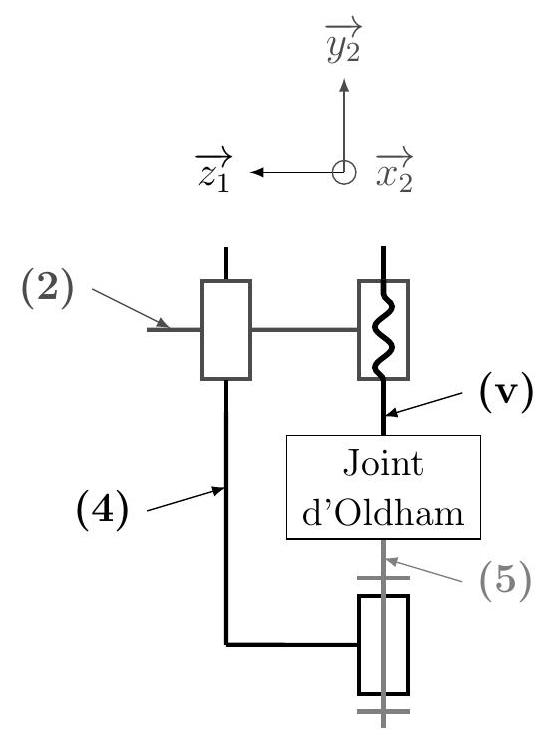
\includegraphics[max width=\textwidth]{2024_04_26_3285cfc264024262add0g-06(1)}
\end{center}

FigURE 6 - Schéma cinématique réduit du mécanisme de déplacement du centre

d'inertie du pendule\\
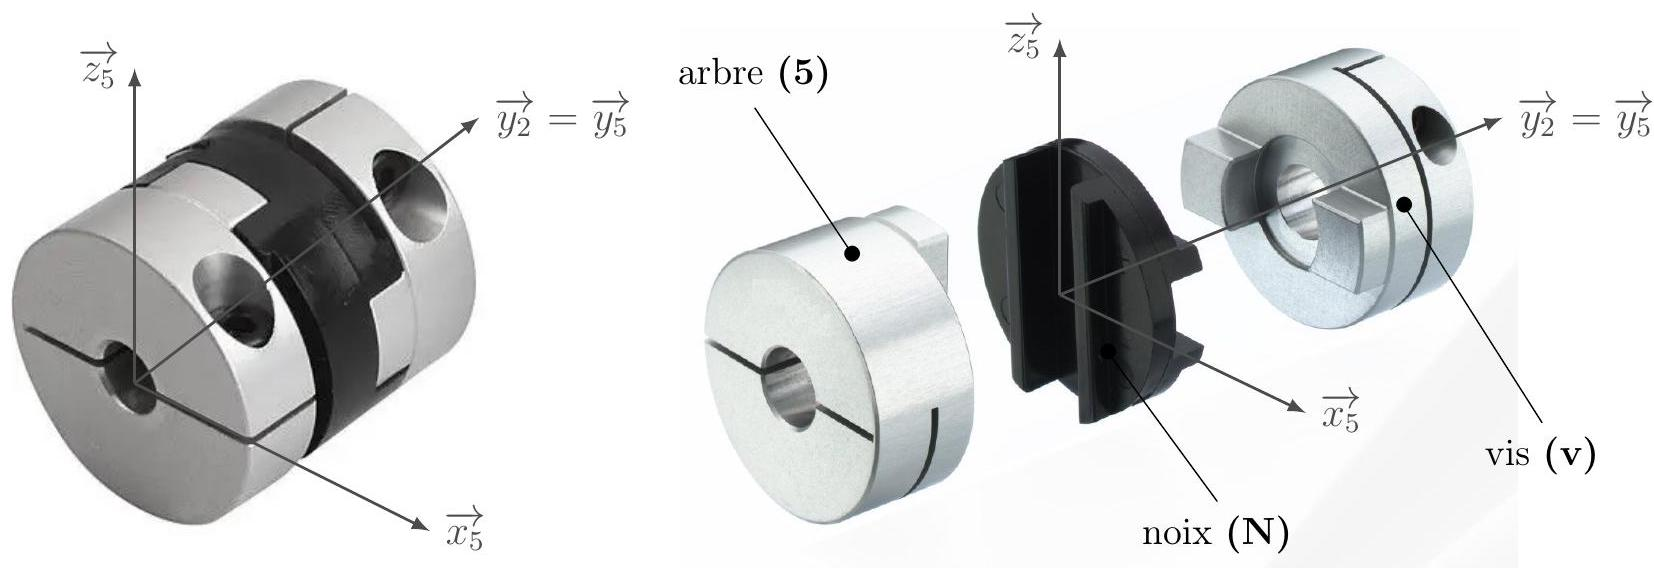
\includegraphics[max width=\textwidth, center]{2024_04_26_3285cfc264024262add0g-06}

FiguRe 7 - Joint d'Oldham assemblé (à gauche) et éclaté (à droite)

Q5. À l'aide de la FigURe 7 et par analyse des surfaces de contact, identifier la liaison entre $(\mathbf{N})$ et (5) d'une part, et entre (N) et (v) d'autre part. Compléter le schéma cinématique en 3D du Cahier Réponses en traçant ces liaisons.

Ce type de joint permet de lier entre eux des éléments d'un mécanisme tout en corrigeant d'éventuels défauts de positionnement relatif entre les arbres (5) et (v).

Q6. Pour chacune des 5 propositions de défauts géométriques du tableau du Cahier Réponses, entourer OUI lorsque le joint d'Oldham permet de rattraper le défaut et entourer NON lorsque ce n'est pas le cas.

\subsection*{2.3 Validation de la précision du positionnement du centre d'inertie du pendule}
\begin{center}
\begin{tabular}{|c|l|l|c|}
\hline
Id & Exigence & Critère & Niveau \\
\hline
$\mathbf{1}$ & Ajuster la position d'équilibre du pendule sur Mars &  &  \\
\hline
$\mathbf{1 . 1}$ & Déplacer le centre d'inertie du pendule & Précision du positionnement & $\pm 3 \mu \mathrm{m}$ \\
\hline
\end{tabular}
\end{center}

TABLE 1 - Liste (non exhaustive) des exigences du mécanisme de translation du centre d'inertie du pendule

Objectif : vérifier que l'exigence 1.1 de précision du positionnement du centre d'inertie du pendule est bien validée.

On introduit, pour le vecteur vitesse de rotation d'un solide $i$ par rapport à un solide $j$, la notation suivante :

$$
\vec{\Omega}_{i / j} \cdot \overrightarrow{y_{2}}=\omega_{i / j}
$$

Les éléments du mécanisme de transformation de mouvement permettant le déplacement du centre d'inertie du pendule sont rappelés en FIGURE 8. Leurs caractéristiques y sont précisées.

\begin{center}
\begin{tabular}{|c|c|c|c|c|c|c|}
\hline
\begin{tabular}{r}
Mot \\
$N_{m}$ \\
\end{tabular} & $\omega_{m}$ & \begin{tabular}{l}
Train \\
4 éta \\
\end{tabular} & $\omega_{5}$ & \begin{tabular}{c}
Joint \\
d'Oldham \\
\end{tabular} & $\omega$ & \begin{tabular}{r}
$\mathrm{V}$ \\
pas $p_{v}$ \\
\end{tabular} \\
\hline
\end{tabular}
\end{center}

FigURE 8 - Chaîne de transmission réalisant le déplacement de la position du centre d'inertie du pendule

Le joint d'Oldham est homocinétique, c'est-à-dire que la vitesse de rotation de l'arbre de sortie du réducteur (5) est la même que celle de la vis (v) par rapport au pendule (2) :

$$
\omega_{5 / 2}=\omega_{v / 2}
$$

Le réducteur est à train épicycloïdal. Son schéma complet est fourni en Annexe 3. Comme il est composé de 4 étages identiques, on résume son étude à celle d'un seul étage, ici le dernier, de manière à en déduire par la suite le rapport de transmission global du train complet. Le schéma cinématique du dernier étage du réducteur est fourni en FIGURE 9 page suivante.

Q7. Justifier que $\omega_{4 / 2}=0$. Établir l'expression du rapport de transmission d'un étage $k=\frac{\omega_{5 / 2}}{\omega_{7 / 2}}$ en fonction des nombres de dents $Z_{i}$ et faire l'application numérique.

\begin{center}
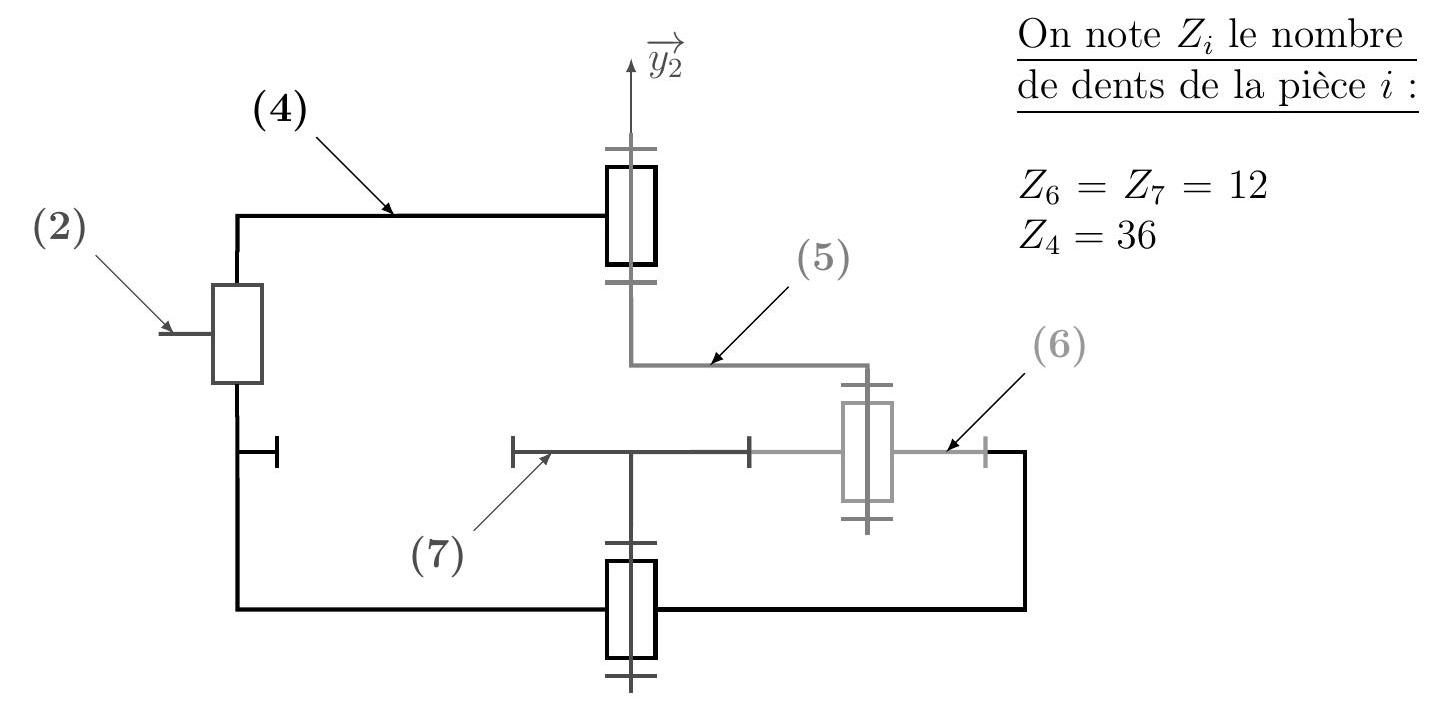
\includegraphics[max width=\textwidth]{2024_04_26_3285cfc264024262add0g-08}
\end{center}

FigURe 9 - Schéma cinématique du dernier étage du train épicycloïdal

Q8. Exprimer le rapport de transmission global du réducteur $k_{g}=\frac{\omega_{5 / 2}}{\omega_{m / 2}}$ en fonction de $k$.

Q9. En s'appuyant sur les notations et données de la FigURE 8, établir l'expression du déplacement linéaire $d_{v}$ de la vis (v) par pas du moteur en fonction de $N_{m}, k_{g}$ et $p_{v}$. Faire l'application numérique et conclure vis-à-vis de l'exigence 1.1 de précision du positionnement du centre d'inertie.

Un capteur optique a permis de mesurer le déplacement de la vis, fourni en FigURE 10, et a mis en évidence une non-linéarité lors des changements de sens de rotation du moteur.\\
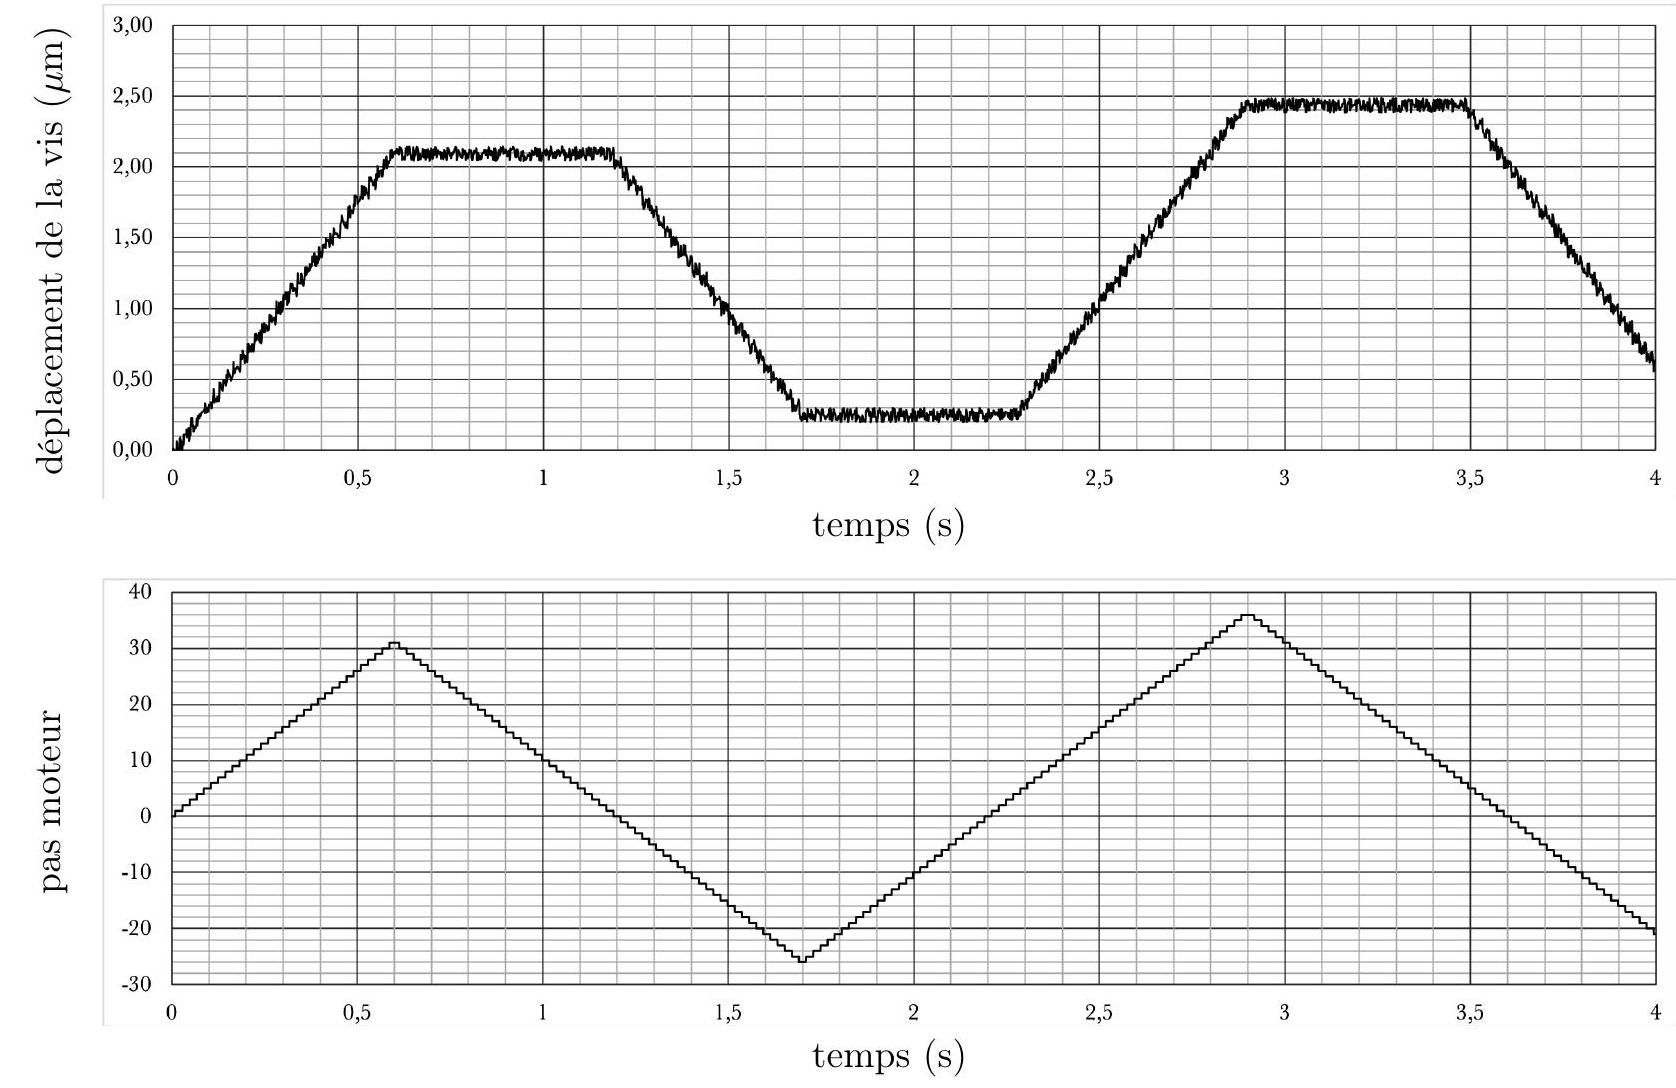
\includegraphics[max width=\textwidth, center]{2024_04_26_3285cfc264024262add0g-08(1)}

FigURe 10 - Déplacement de la vis en $\mu \mathrm{m}$ et nombre de pas du moteur en fonction du temps

Q10. Proposer une cause de la non-linéarité qui apparait au changement de sens de rotation du moteur.

Q11. Donner l'erreur de positionnement due à la non-linéarité. Conclure à nouveau vis-à-vis de l'exigence 1.1 de précision du positionnement du centre d'inertie.

\section*{3 Caractérisation dynamique de l'ensemble mobile}
On rappelle que les pendules inversés du sismomètre VBB conservent leur équilibre autour de leur axe de rotation $\left(O_{1}, \overrightarrow{z_{1}}\right)$ par rapport au bâti grâce à un ressort à lame souple. Afin que chaque système soit suffisamment sensible aux séismes sur Mars, le choix du ressort associé à une articulation à lamelles doit également permettre d'amplifier les mouvements sur la plage de fréquences attendues pour les séismes martiens.

On définit pour cela les exigences de la TABLE 2.

\begin{center}
\begin{tabular}{|c|l|l|c|}
\hline
$\mathbf{2}$ & Être mécaniquement sensible aux séismes attendus sur Mars &  &  \\
\hline
$\mathbf{2 . 1}$ & Être suffisamment sensible & Amplification mécanique & $>2 \mathrm{rad} \cdot \mathrm{m}^{-1} \cdot \mathrm{s}^{2}$ \\
\hline
$\mathbf{2 . 2}$ & \begin{tabular}{l}
Être sensible aux fréquences des \\
séismes attendus sur Mars \\
\end{tabular} & \begin{tabular}{l}
Amplification en fonction de \\
la fréquence des mouvements \\
du sol \\
\end{tabular} & \begin{tabular}{c}
$\geq 10 \mathrm{~dB}$ dans la bande \\
$[0,01 ; 0,5] \mathrm{Hz}$ \\
soit $[0,06 ; 3] \mathrm{rad} \cdot \mathrm{s}^{-1}$ \\
\end{tabular} \\
\hline
\end{tabular}
\end{center}

TABLE 2 - Liste (non exhaustive) des exigences de sensibilité mécanique d'un système

Chaque ressort est unique, et entre les trois systèmes constituant VBB, ces derniers ne sont pas interchangeables. Ils sont fabriqués sur mesure, en tenant compte des caractéristiques des articulations à lamelles, uniques elles aussi.

Objectif : établir le lien entre la raideur du ressort et la pulsation propre de l'ensemble mobile; choisir un ressort et une articulation à lamelles de façon à respecter les exigences 2.1 et 2.2.

\subsection*{3.1 Modélisation dynamique de l'ensemble mobile en réponse à un séisme}
En cas de séisme, le sol (1) est en mouvement. Il entraîne dans son mouvement le bâti du système et ne peut plus être considéré comme un référentiel galiléen.

Le schéma cinématique et le paramétrage du dispositif sont fournis en Annexe 4, ainsi que l'ensemble des notations et hypothèses utiles pour cette sous-partie.

On admet qu'il y a un mouvement de translation de (1) par rapport au repère $R_{0}$ dans les directions $\overrightarrow{x_{1}}$ et $\overrightarrow{y_{1}}$, comme imposé par les deux liaisons glissières en série entre (1) et $R_{0}$ sur le schéma cinématique de l'Annexe 4. Aucun degré de liberté en rotation n'est admis : $\vec{\Omega}_{1 / 0}=\overrightarrow{0}$.

Un logiciel de CAO a permis de déterminer numériquement la matrice d'inertie du pendule (2) équipé du contrepoids (3) en $O_{1}$, où tous les termes sont en $\mathrm{kg} \cdot \mathrm{m}^{2}$ :

$$
\overline{\bar{I}}_{\left(O_{1}, 2+3\right)}=\left(\begin{array}{ccc}
5,31 \times 10^{-4} & -0,94 \times 10^{-4} & -5,67 \times 10^{-7} \\
-0,94 \times 10^{-4} & 1,25 \times 10^{-4} & -2,33 \times 10^{-8} \\
-5,67 \times 10^{-7} & -2,33 \times 10^{-8} & 4,04 \times 10^{-4}
\end{array}\right)_{\left(\overrightarrow{x_{2}}, \overrightarrow{y_{2}}, \overrightarrow{z_{1}}\right)}=\left(\begin{array}{ccc}
I_{x x} & -I_{x y} & -I_{x z} \\
-I_{x y} & I_{y y} & -I_{y z} \\
-I_{x z} & -I_{y z} & I_{z z}
\end{array}\right)_{\left(\overrightarrow{\left.x_{2}, \overrightarrow{y_{2}}, \overrightarrow{z_{1}}\right)}\right.}
$$

Q12. Quel plan de symétrie de l'ensemble mobile $\{(2)+(3)\}$ serait cohérent avec les valeurs numériques de la matrice d'inertie $\overline{\bar{I}}_{\left(O_{1}, 2+3\right)}$ déterminée par le logiciel de CAO ? En déduire, sous sa forme littérale, l'écriture simplifiée de la matrice d'inertie.

Q13. Déterminer, dans son mouvement par rapport au repère $R_{0}$, l'expression du moment cinétique de $\{(\mathbf{2})+(3)\}$ en $O_{1}, \vec{\sigma}_{O_{1},(2+3) / R_{0}}$. On l'exprimera en fonction des paramètres cinétiques de $\{(2)+(3)\}$ et des paramètres géométriques et cinématiques du système.

Q14. Montrer que la projection sur $\overrightarrow{z_{1}}$ du moment dynamique de $\{(2)+(3)\}$ dans son mouvement par rapport au repère $R_{0}$ en $O_{1}$, est de la forme suivante :

$$
\vec{\delta}_{O_{1},(2+3) / R_{0}} \cdot \overrightarrow{z_{1}}=I_{z z} \ddot{\alpha}(t)-d M \gamma_{x 2}(t)
$$

où l'on précisera l'expression de $\gamma_{x 2}(t)$.

On déduit de cette équation que $\overrightarrow{x_{2}}$ est la direction de sensibilité de l'ensemble mobile, c'est-à-dire que l'ensemble mobile n'est sensible qu'aux accélérations du sol en projection sur $\overrightarrow{x_{2}}$.

Q15. Préciser, sans faire de calculs, le système isolé et l'équation issue du Principe Fondamental de la Dynamique qui permet d'obtenir l'équation du mouvement de l'ensemble mobile suivante :


\begin{equation*}
I_{z z} \ddot{\alpha}(t)+\mu \dot{\alpha}(t)+k\left(\alpha(t)-\alpha_{0}\right)=a M_{2} g_{\mathrm{M}} \sin \alpha(t)+d M \gamma_{x 2}(t)+C_{0} \tag{eq.2}
\end{equation*}


Donner les éléments d'application (équation, projection, point éventuel...) du théorème utilisé. Justifier que l'équation obtenue n'est pas linéaire, indépendamment de l'expression de $\gamma_{x 2}(t)$.

Afin de mettre en évidence les caractéristiques de l'ensemble mobile en réponse à une accélération du sol $\gamma_{x 2}(t)$, ses oscillations ayant une amplitude très faible, l'équation du mouvement est linéarisée autour du point d'équilibre $\alpha_{\mathrm{eq}}=\alpha_{0}$ de l'ensemble mobile.

On pose $\alpha(t)=\alpha_{0}+\Delta \alpha(t)$, avec $\Delta \alpha(t) \ll \alpha_{0}$.

Q16. Montrer que l'équation du mouvement linéarisée s'écrit :


\begin{equation*}
I_{z z} \ddot{\Delta} \alpha(t)+\mu \dot{\Delta} \alpha(t)+k \Delta \alpha(t)=a M_{2} g_{\mathrm{M}} \cos \alpha_{0} \Delta \alpha(t)+d M \gamma_{x 2}(t) \tag{eq.3}
\end{equation*}


On note $\alpha(p)$ et $\gamma_{x 2}(p)$ respectivement les transformées de Laplace des variations angulaires $\Delta \alpha(t)$ et de l'accélération du sol $\gamma_{x 2}(t)$. Les conditions initiales sont supposées nulles.

Q17. Exprimer, sous forme canonique, la fonction de transfert de l'ensemble mobile $\frac{\alpha(p)}{\gamma_{x 2}(p)}$ et donner la condition de stabilité de l'ensemble mobile sous la forme d'une inéquation. Conclure sur le rôle stabilisateur du ressort.

Q18. Donner, en fonction des constantes du problème, les expressions des constantes caractéristiques de cette fonction de transfert : gain d'amplification mécanique noté $A$, pulsation propre $\omega_{0}$ et coefficient d'amortissement $\xi$.

\subsection*{3.2 Choix du couple ressort/articulation pour le système}
Pour optimiser la conception des systèmes, 50 ressorts à lame souple et 8 articulations à lamelles ont été fabriqués. L'association d'un ressort et d'une articulation confère une certaine raideur $k$ et un certain moment de précontrainte $C_{0}$ sur l'axe de rotation du pendule par rapport au bâti. Grâce au dispositif expérimental mis au point avec le contrepoids, $k$ et $C_{0}$ sont mesurés pour chaque association, ce qui permet de tracer point par point le diagramme de la FIGURE A du Cahier Réponses. Pour faciliter l'interprétation du diagramme, seuls 16 points ont été tracés au lieu de 400 .

Le couple idéal ressort/articulation doit être déterminé pour une utilisation du pendule sur Mars, c'est-à-dire sans contrepoids. Ainsi, les équations précédentes $(1,1,2$ et 3 ) restent valables, en substituant $M_{2}$ par $M$ et $a$ par $d$.

De plus, $\alpha_{\mathrm{eq}}=\alpha_{0}$. On admet que $\alpha_{0}=30^{\circ}$ assure un bon compromis entre un gain d'amplification maximisé et un bruit de mesure faible.

Les données numériques utiles sont résumées dans le tableau suivant, dans les Unités du Système International (USI) :

\begin{center}
\begin{tabular}{|c|c|c|}
\hline
$d M$ & $g_{M}$ & $d M g_{\mathrm{M}} \cos \alpha_{0}$ \\
\hline
$4,4 \times 10^{-3} \mathrm{~m} \cdot \mathrm{kg}$ & $4 \mathrm{~m} \cdot \mathrm{s}^{-2}$ & $15 \times 10^{-3} \mathrm{USI}$ \\
\hline
\end{tabular}
\end{center}

Q19. Déterminer la valeur numérique de $C_{0}$ pour assurer l'équilibre du pendule.

Q20. Donner les 2 inéquations qui régissent le choix de la raideur $k$ du couple ressort/articulation, afin de satisfaire l'exigence 2.1 et d'avoir un système stable. À l'aide d'applications numériques, en déduire la plage de valeurs acceptables pour $k$ afin de satisfaire ces 2 conditions.

Q21. Sur la FiguRe A du Cahier Réponses, tracer les droites encadrant les valeurs acceptables pour $k$ et la droite correspondant à la valeur idéale de $-C_{0}$. En déduire le meilleur couple ressort/articulation pour le pendule étudié en entourant le point correspondant sur le diagramme.

Le diagramme de Bode en gain de la fonction de transfert $\frac{\alpha(p)}{\gamma_{x 2}(p)}$ du système pour ce choix du couple ressort/articulation est fourni sur la FiguRe B du Cahier Réponses.

Q22. Conclure vis-à-vis de l'exigence 2.2. Les tracés nécessaires devront figurer sur la FIGURE B du Cahier Réponses. Le système en l'état est-il satisfaisant pour la mesure des mouvements du sol martien dans la plage de fréquence des séismes attendus sur Mars?

\section*{4 Performances de l'asservissement}
À chaque mouvement du sol, un capteur mesure la position angulaire du pendule (2) par rapport au bâti (1). Des bobines de contre-réaction situées sur le pendule (voir FIGURE 2 et l'Annexe 1) génèrent un moment de rappel sur son axe de rotation, qui le ramène à sa position d'équilibre.

\begin{itemize}
  \item La bobine HF (pour Haute Fréquence) pilote l'asservissement entre 0,05 Hz et 0,5 Hz. Son rôle principal est d'amortir les secousses trop brusques et d'éliminer la résonance du pendule.
  \item La bobine BF (pour Basse Fréquence) a été conçue pour intervenir sur les fréquences inférieures à $0,05 \mathrm{~Hz}$. Elle permet de filtrer la variation journalière de température et les dérives saisonnières plus lentes.
\end{itemize}

L'asservissement mis en place est donc une régulation devant permettre d'annuler en régime permanent les effets des secousses sismiques sur le pendule, tout en étant sensible aux signaux dans une large bande de fréquences d'ondes sismiques, entre $0,01 \mathrm{~Hz}$ et $0,5 \mathrm{~Hz}$.

Les exigences auxquelles doit répondre cet asservissement sont fournies dans la TABLE 3.

\begin{center}
\begin{tabular}{|c|l|l|c|}
\hline
$\mathbf{3}$ & Acquérir les vibrations du sol martien &  &  \\
\hline
$\mathbf{3 . 1}$ & \begin{tabular}{l}
Éliminer la résonance du \\
système tout en maintenant une \\
rapidité maximale \\
\end{tabular} & \begin{tabular}{l}
Résonance du système avec \\
l'action de la bobine HF seule \\
\end{tabular} & aucune \\
\cline { 3 - 4 }
\begin{tabular}{l}
Rapidité du système avec l'ac- \\
tion de la bobine HF seule \\
\end{tabular} & \begin{tabular}{c}
bande passante à $-3 \mathrm{~dB}$ \\
maximale \\
\end{tabular} &  &  \\
\hline
$\mathbf{3 . 2}$ & \begin{tabular}{l}
Ramener le déplacement du pen- \\
dule à zéro \\
\end{tabular} & \begin{tabular}{l}
Précision de l'asservissement \\
en tension \\
\end{tabular} & \begin{tabular}{c}
écart statique nul en \\
réponse à un échelon \\
d'accélération du sol \\
\end{tabular} \\
\hline
$\mathbf{3 . 3}$ & Filtrer le signal & \begin{tabular}{l}
Amplification des mouve- \\
ments du sol par l'asservisse- \\
ment en tension \\
\end{tabular} & \begin{tabular}{c}
$\geq 110 \mathrm{~dB}$ limitée à la \\
bande $[0,06 ; 3]$ rad $\mathrm{s}^{-1}$ \\
\end{tabular} \\
\hline
$\mathbf{3 . 4}$ & \begin{tabular}{l}
Éviter des problèmes de satura- \\
tion \\
\end{tabular} & \begin{tabular}{l}
Amplification des mouve- \\
ments du sol par l'asservisse- \\
ment en tension \\
\end{tabular} & \begin{tabular}{c}
$<120 \mathrm{~dB}$ pour tous les \\
signaux mesurés \\
\end{tabular} \\
\hline
\end{tabular}
\end{center}

TABLE 3 - Liste (non exhaustive) des exigences de l'asservissement

Objectif : régler la correction des bobines $\mathrm{HF}$ et $\mathrm{BF}$.

Le réglage de l'asservissement s'effectue par une étude numérique, dans les conditions de la gravité martienne. On considère donc le pendule (2) sans son contrepoids (3). On note $J$ le moment d'inertie du pendule (2) sur l'axe ( $\left.O_{1}, \overrightarrow{z_{1}}\right)$. Pour simplifier l'étude, on néglige les frottements dans l'articulation à lamelles, et on note $K=k-d M g_{M} \cos \alpha_{0}$ la raideur équivalente du pendule.

La grandeur utile aux scientifiques qui analysent les données mesurées par le sismomètre est la tension électrique en sortie du capteur, image de la position angulaire du pendule autour de sa position d'équilibre.

Le schéma-blocs de l'asservissement en tension d'un système est fourni en Annexe 5 , ainsi que la description des grandeurs physiques intervenant dans l'asservissement et les données numériques utiles à cette partie.

On s'intéresse dans un premier temps à l'asservissement avec l'action de la bobine HF seule. Le schéma-blocs correspondant est fourni à la FIGURE 11.

\begin{center}
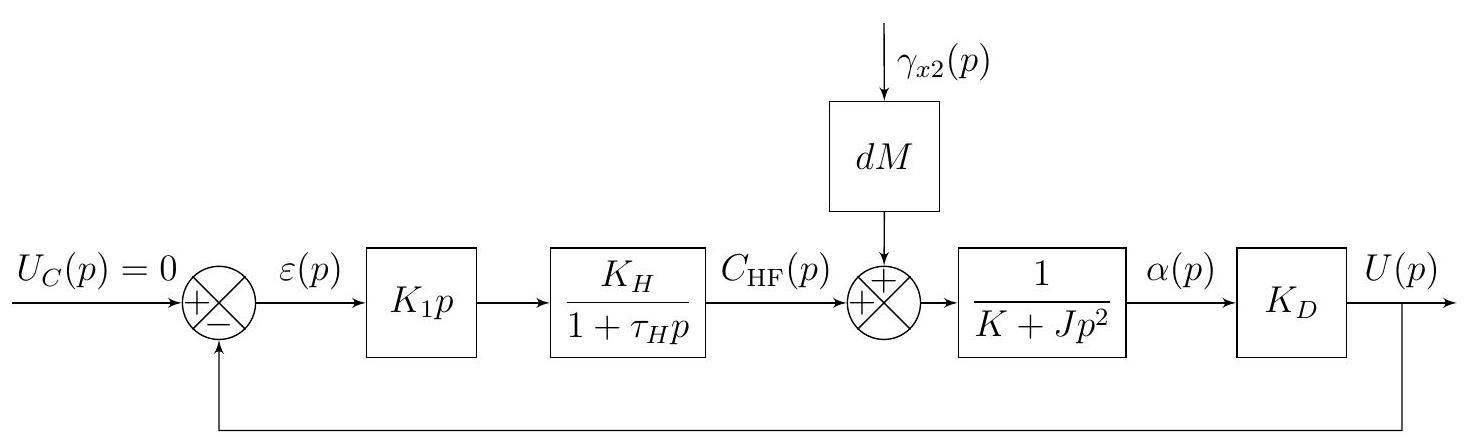
\includegraphics[max width=\textwidth]{2024_04_26_3285cfc264024262add0g-13(1)}
\end{center}

FIGURE 11 - Schéma-blocs de l'asservissement avec l'action de la bobine HF seule

Q23. Déterminer la fonction de transfert $H_{\gamma}(p)=\frac{U(p)}{\gamma_{x 2}(p)}$, avec $U_{C}(p)=0$, en l'exprimant sous la forme:

$$
H_{\gamma}(p)=K_{\mathrm{HF}} \cdot \frac{1+a_{1} p}{1+b_{1} p+b_{2} p^{2}+b_{3} p^{3}}
$$

où l'on précisera les expressions de $K_{\mathrm{HF}}, a_{1}, b_{1}, b_{2}$ et $b_{3}$.

On donne les pôles $p_{i}$ de $H_{\gamma}(p)$ en TABLE 4 et le diagramme de Bode en gain de $H_{\gamma}(p)$ en FigURe 12 pour différentes valeurs de $K_{1}$.

\begin{center}
\begin{tabular}{|c|c|c|c|}
\hline
$K_{1}$ & $p_{1}$ & $p_{2}$ & $p_{3}$ \\
\hline\hline
0,05 & -1000 & $-0,38-2,33 \mathrm{j}$ & $-0,38+2,33 \mathrm{j}$ \\
\hline
0,5 & -1000 & $-0,64$ & $-9,32$ \\
\hline
5 & -1000 & $-0,069$ & $-95,7$ \\
\hline
\end{tabular}
\end{center}

TABLE 4 - Pôles de la fonction de transfert $H_{\gamma}(p)$

\begin{center}
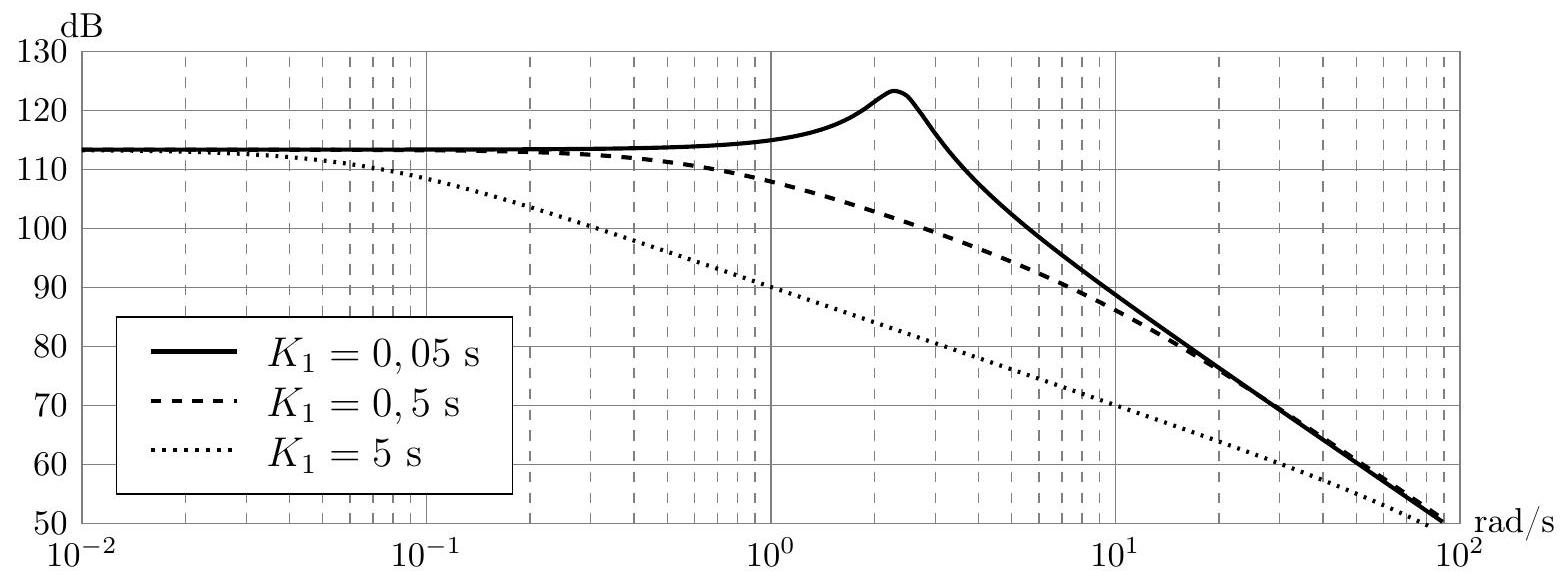
\includegraphics[max width=\textwidth]{2024_04_26_3285cfc264024262add0g-13}
\end{center}

Figure 12 - Diagramme de Bode en gain de la fonction de transfert $H_{\gamma}(p)$

Le réglage du correcteur HF doit permettre de répondre à l'exigence 3.1.

Q24. Justifier que $H_{\gamma}(p)$ correspond à un système stable quelle que soit la valeur retenue pour $K_{1}$ dans la gamme $[0,05 ; 5]$ s. Choisir, en justifiant, la valeur de $K_{1}$ parmi les valeurs proposées, la plus adaptée au réglage de l'asservissement avec l'action de la bobine HF seule.

Q25. En s'appuyant sur les données numériques de la TABLE 4 et de l'Annexe 5, justifier que, pour la valeur retenue de $K_{1}$, la fonction de transfert peut s'écrire sous la forme :

$$
H_{\gamma}(p)=\frac{d M K_{D}}{K} \cdot \frac{1}{\left(1+\tau_{2} p\right)\left(1+\tau_{3} p\right)}, \text { avec } \tau_{2} \gg \tau_{3}
$$

Préciser les valeurs des constantes de temps $\tau_{2}$ et $\tau_{3}$.

Pour la suite des questions, on conservera cette forme simplifiée de $H_{\gamma}(p)$.

Q26. Justifier que l'asservissement avec l'action de la bobine HF seule ne permet pas de satisfaire les exigences 3.2 et 3.3 .

En tenant compte des résultats précédents, le schéma-blocs de l'Annexe 5 peut se mettre sous la forme de celui de la Figure 13.

\begin{center}
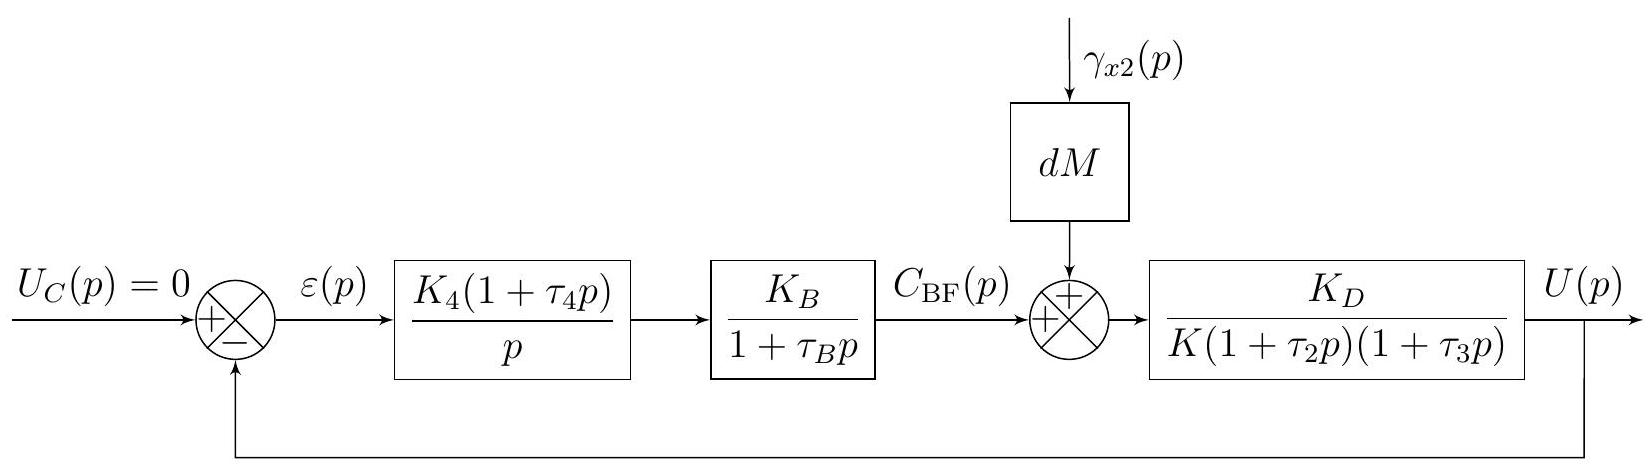
\includegraphics[max width=\textwidth]{2024_04_26_3285cfc264024262add0g-14}
\end{center}

FigURe 13 - Schéma-blocs de l'asservissement d'un système

Le correcteur BF est un correcteur proportionnel intégral. Pour optimiser la rapidité, $\tau_{4}$ doit permettre de compenser le pôle dominant de la boucle ouverte. $K_{4}$ est réglé de façon à répondre aux exigences 3.3 et 3.4.

Q27. Préciser l'intérêt de la chaîne d'action BF vis-à-vis de l'exigence 3.2.

Q28. Donner l'expression de la fonction de transfert en boucle ouverte de l'asservissement, $H_{B O}(p)=\frac{U(p)}{\varepsilon(p)}$. Donner, en justifiant, la valeur retenue pour $\tau_{4}$.

On donne, pour la valeur de $\tau_{4}$ retenue et différentes valeurs de $K_{4}$, le diagramme de Bode de l'asservissement en tension, $\frac{U(p)}{\gamma_{x 2}(p)}$, sur la FiguRE C du Cahier Réponses.

Q29. Choisir, en justifiant, la valeur de $K_{4}$ qui permet de vérifier au mieux les exigences 3.3 et 3.4. Les tracés nécessaires apparaitront sur la FiguRe $\mathrm{C}$ du Cahier Réponses.

Q30. Donner le nom du type de filtre réalisé par le pendule asservi et préciser l'intérêt de cette solution pour la mesure des séismes par le sismomètre VBB.

\section*{Annexe 1 - Détail des éléments d'un des systèmes du VBB}
\begin{center}
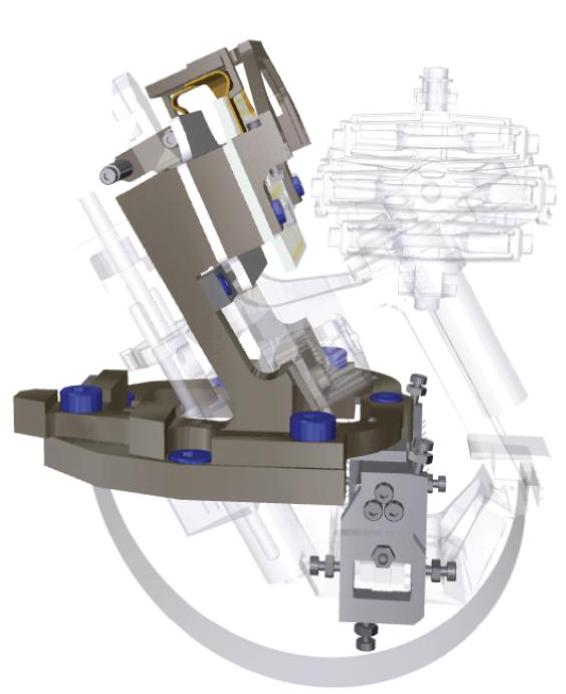
\includegraphics[max width=\textwidth]{2024_04_26_3285cfc264024262add0g-15(3)}
\end{center}

bâti (1)

\begin{center}
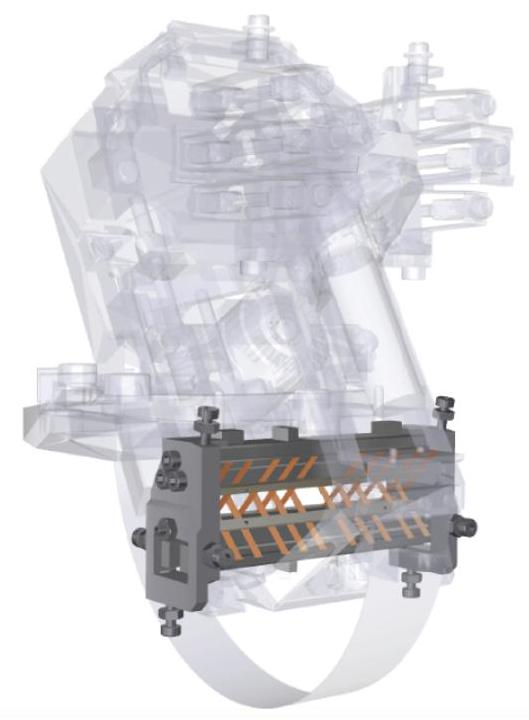
\includegraphics[max width=\textwidth]{2024_04_26_3285cfc264024262add0g-15(2)}
\end{center}

articulation à lamelles entre (1) et (2)

\begin{center}
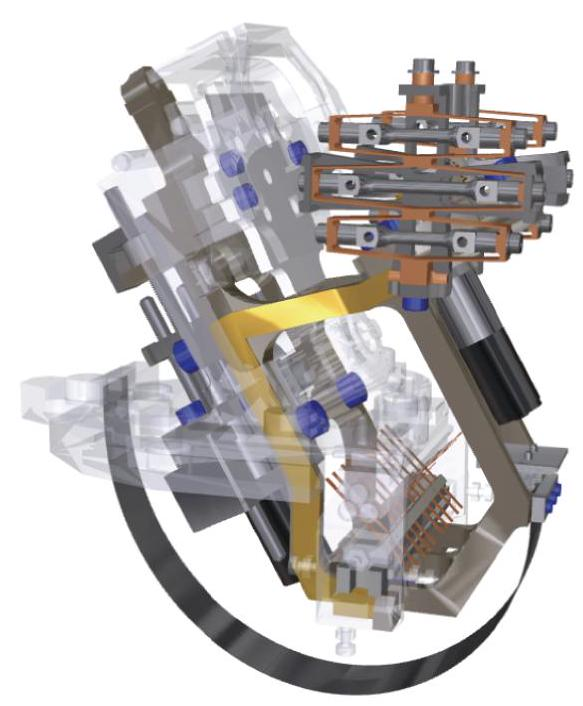
\includegraphics[max width=\textwidth]{2024_04_26_3285cfc264024262add0g-15}
\end{center}

pendule (2)

\begin{center}
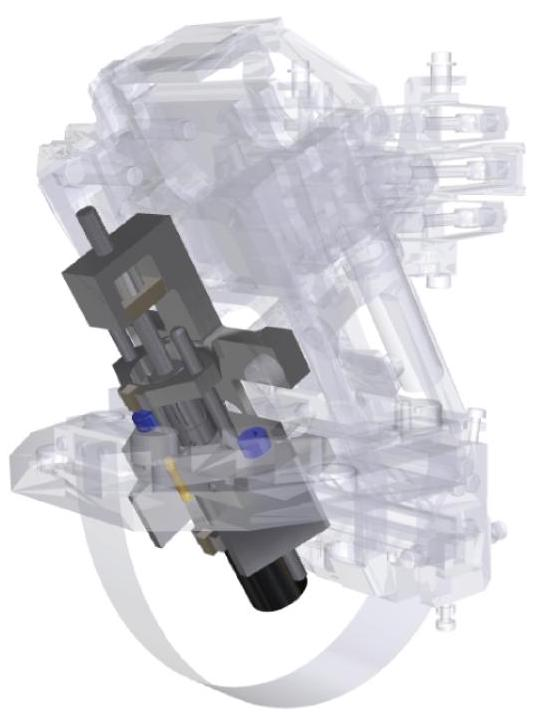
\includegraphics[max width=\textwidth]{2024_04_26_3285cfc264024262add0g-15(1)}
\end{center}

mécanisme de translation du centre d'inertie de (2)

\section*{Annexe 2 - Modèle cinématique du système en l'absence de séisme}
\begin{center}
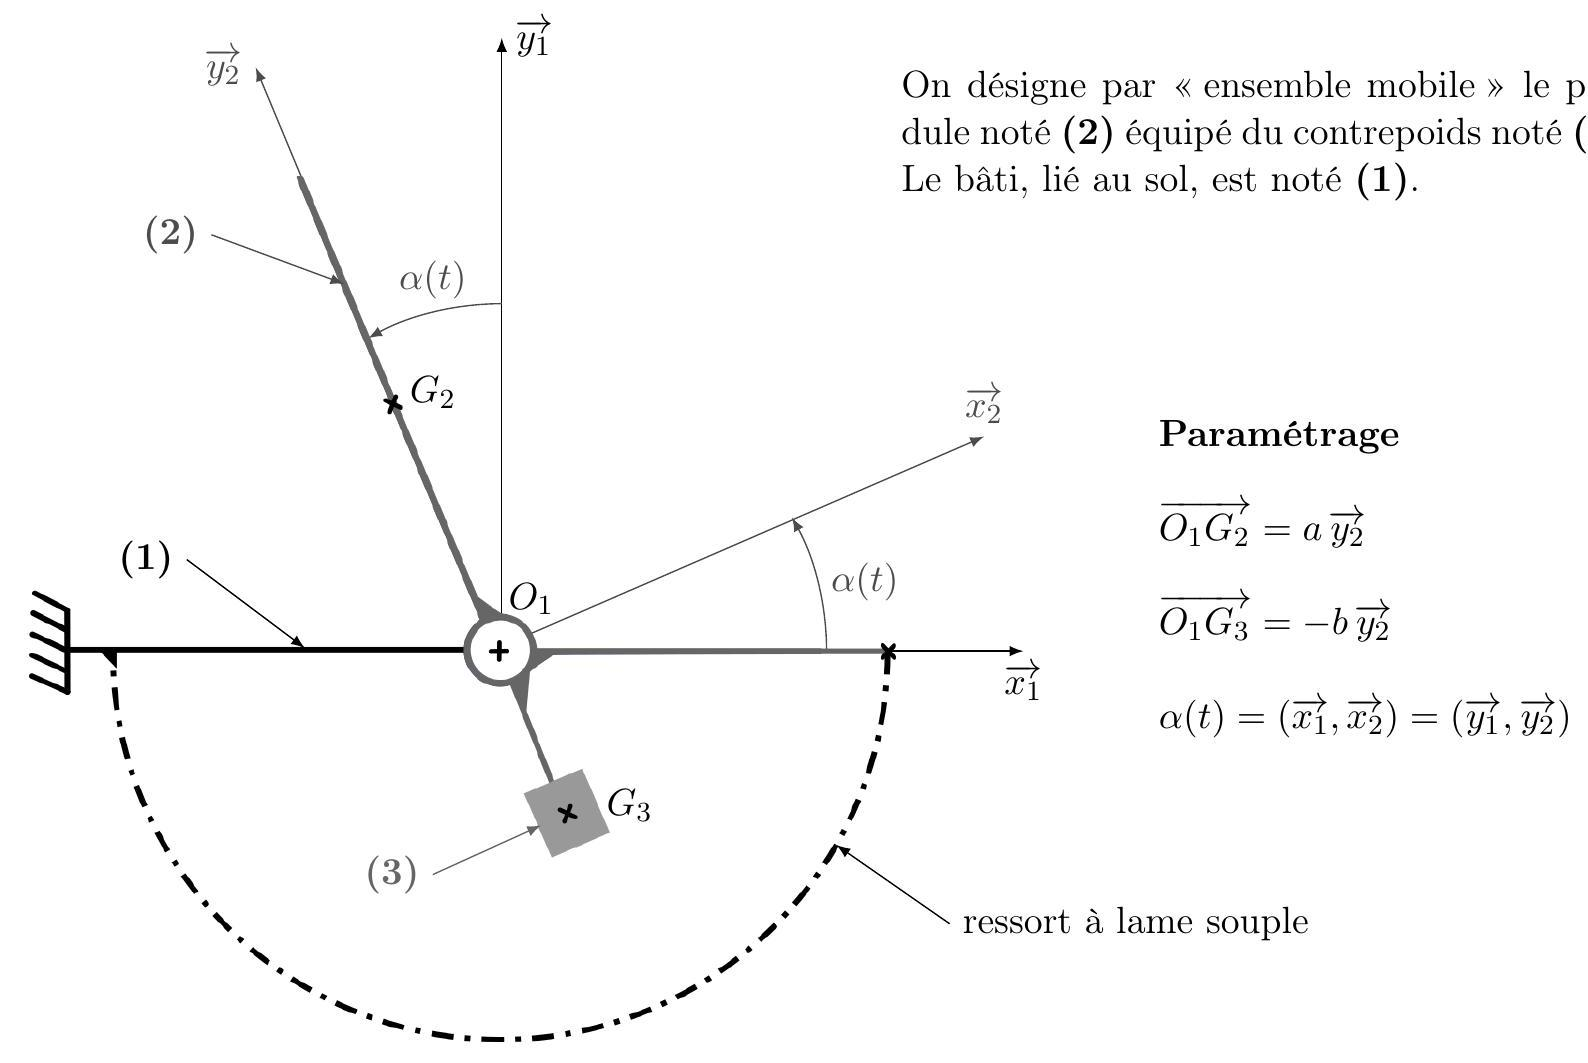
\includegraphics[max width=\textwidth]{2024_04_26_3285cfc264024262add0g-16}
\end{center}

\section*{Notations}
\begin{center}
\begin{tabular}{|c|l|}
\hline
$G_{2}$ & centre d'inertie du pendule (2) \\
\hline
$M_{2}$ & masse du pendule (2) \\
\hline
$G_{3}$ & centre d'inertie du contrepoids (3) \\
\hline
$m_{3}$ & masse du contrepoids (3) \\
\hline
$C_{0}$ & \begin{tabular}{l}
moment de précontrainte de l'ensemble \\
\{ressort + articulation $\}$ sur $\{(\mathbf{2})+(\mathbf{3})\}$ \\
\end{tabular} \\
\hline
$k$ & \begin{tabular}{l}
raideur de l'ensemble \{ressort + articu- \\
lation\} sur l'axe $\left(O_{1}, \overrightarrow{z_{1}}\right)$ \\
\end{tabular} \\
\hline
$\alpha_{0}$ & \begin{tabular}{l}
position angulaire à vide de l'ensemble \\
mobile \\
\end{tabular} \\
\hline
$\alpha_{\mathrm{eq}}$ & \begin{tabular}{l}
position angulaire de l'ensemble mobile \\
à l'équilibre (sous l'effet des actions de \\
la pesanteur et du ressort) \\
\end{tabular} \\
\hline
$g_{T}$ & \begin{tabular}{l}
champ de pesanteur à la surface de la \\
Terre, de direction $-\overrightarrow{y_{1}}$ \\
\end{tabular} \\
\hline
$g_{M}$ & \begin{tabular}{l}
champ de pesanteur à la surface de Mars, \\
de direction $-\overrightarrow{y_{1}}$ \\
\end{tabular} \\
\hline
\end{tabular}
\end{center}

\section*{Hypothèses}
Le référentiel $\mathcal{R}_{1}$, auquel est associé le repère $R_{1}=\left(O_{1}, \overrightarrow{x_{1}}, \overrightarrow{y_{1}}, \overrightarrow{z_{1}}\right)$ lié au sol, est supposé galiléen en l'absence de séisme.

La liaison pivot réalisée par l'articulation à lamelle sur l'axe de rotation $\left(O_{1}, \overrightarrow{z_{1}}\right)$ de l'ensemble mobile n'est pas parfaite. Les frottements visqueux sont pris en compte à travers un coefficient de frottement $\mu(\mu>0)$ :

$$
\left\{\mathcal{T}_{1 \rightarrow(2+3)}\right\}=\left\{\begin{array}{c}
X_{O} \overrightarrow{x_{1}}+Y_{O} \overrightarrow{y_{1}}+Z_{O} \overrightarrow{z_{1}} \\
L_{O} \overrightarrow{x_{1}}+M_{O} \overrightarrow{y_{1}}-\mu \dot{\alpha}(t) \overrightarrow{z_{1}}
\end{array}\right\}_{O_{1}}
$$

L'action de rappel de l'ensemble $\{$ ressort + articulation $\}$ est assimilée à un couple pur sur l'axe de rotation $\left(O_{1}, \overrightarrow{z_{1}}\right)$ de l'ensemble mobile :

$\left\{\mathcal{T}_{\text {ressort } \rightarrow(2+3)}\right\}=\left\{\begin{array}{c}\overrightarrow{0} \\ \left(C_{0}-k\left(\alpha(t)-\alpha_{0}\right)\right) \overrightarrow{z_{1}}\end{array}\right\}_{O_{1}}$

Annexe 3 - Schéma cinématique du mécanisme de translation de la position du centre d'inertie du pendule

\begin{center}
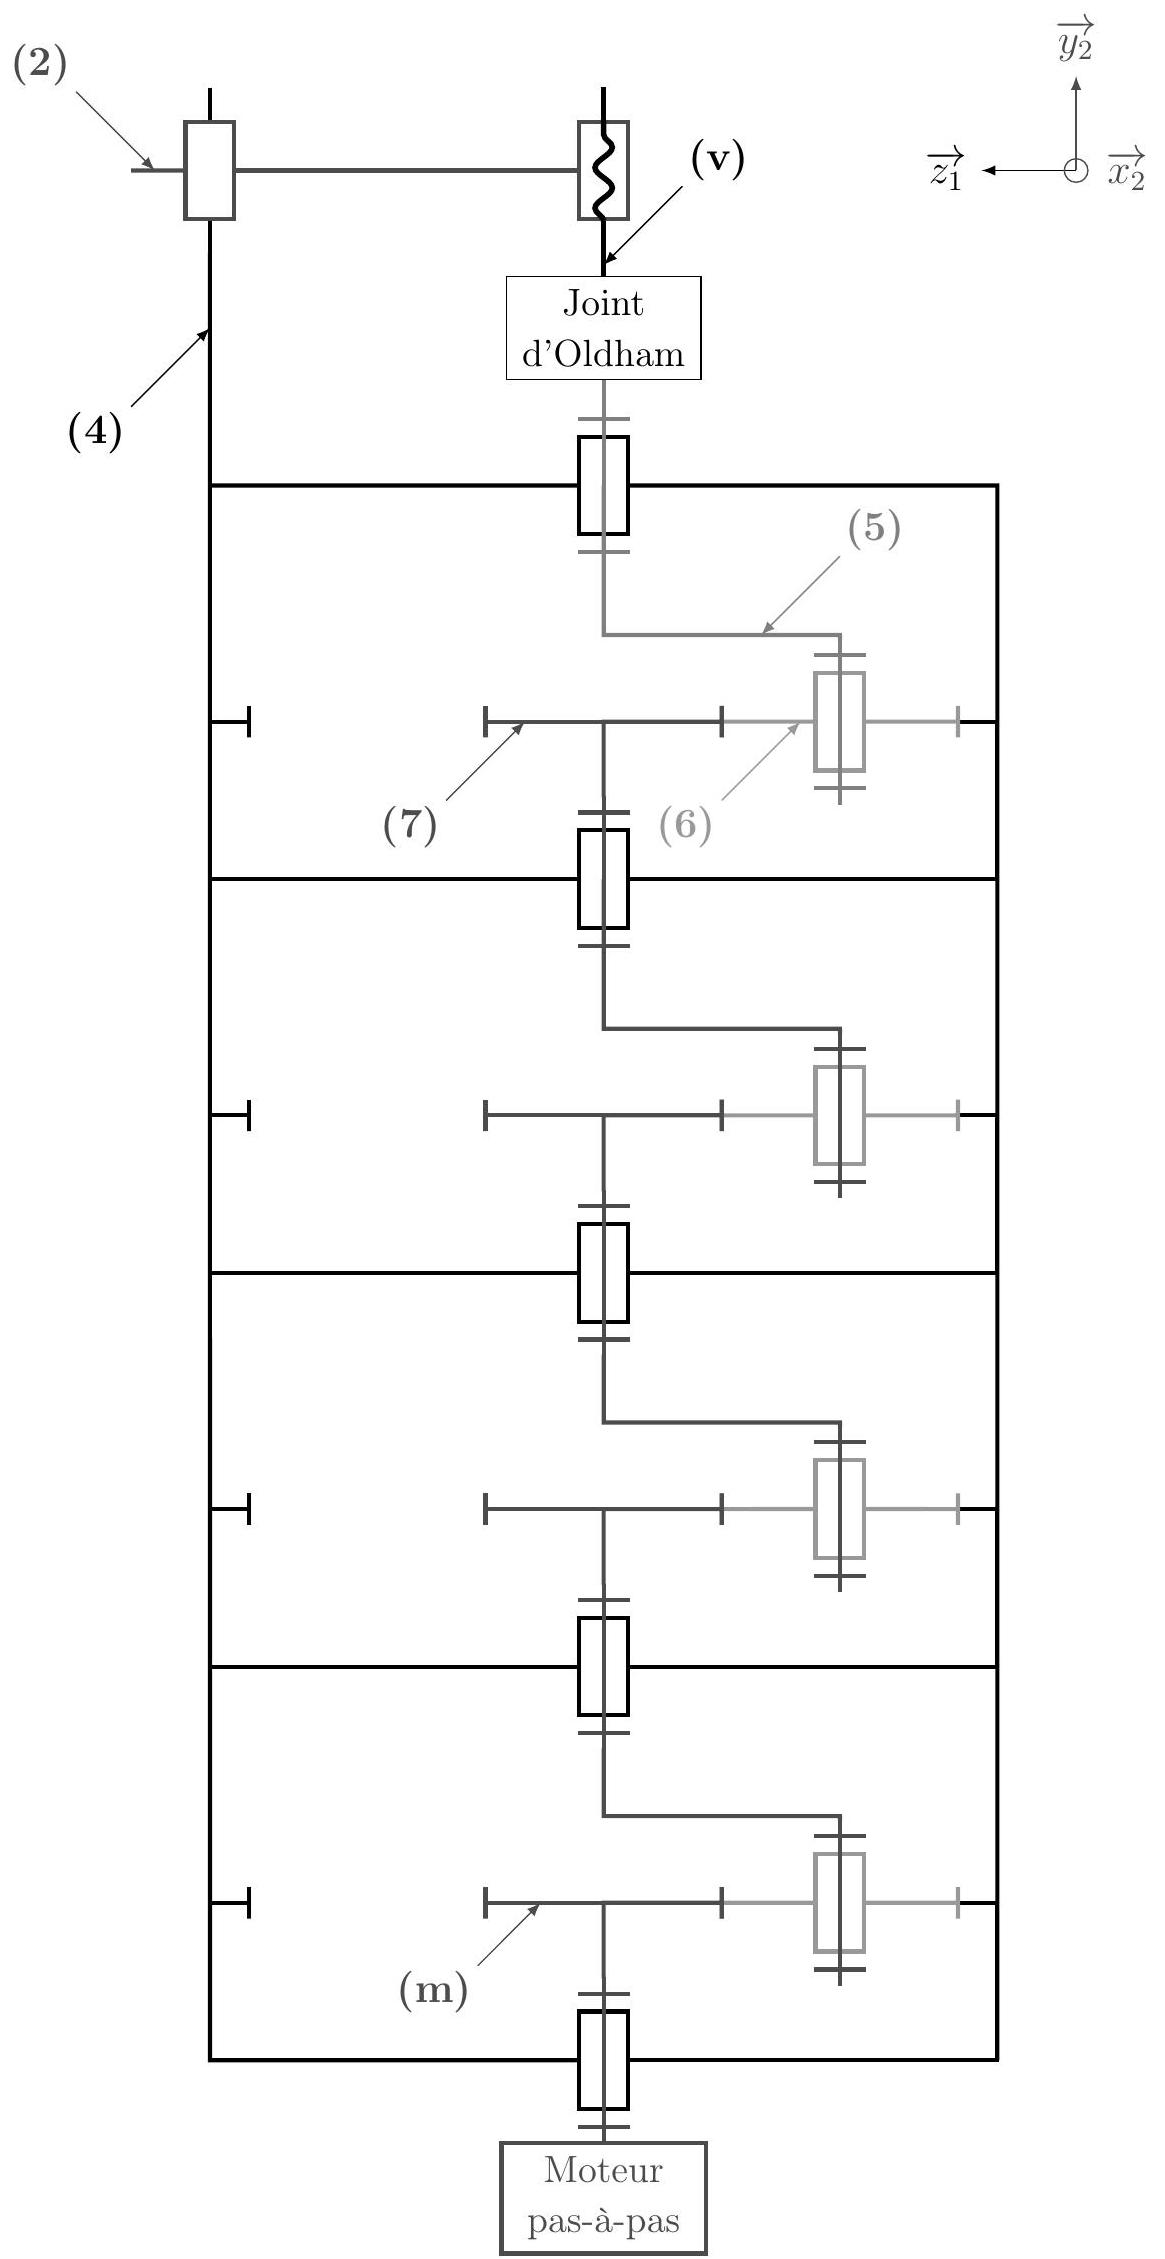
\includegraphics[max width=\textwidth]{2024_04_26_3285cfc264024262add0g-17}
\end{center}

Page $3 / 5$

\section*{Annexe 4 - Modèle cinématique du système lors d'un séisme}
Les torseurs d'actions mécaniques et les notations de l'Annexe 2 restent valables.

\begin{center}
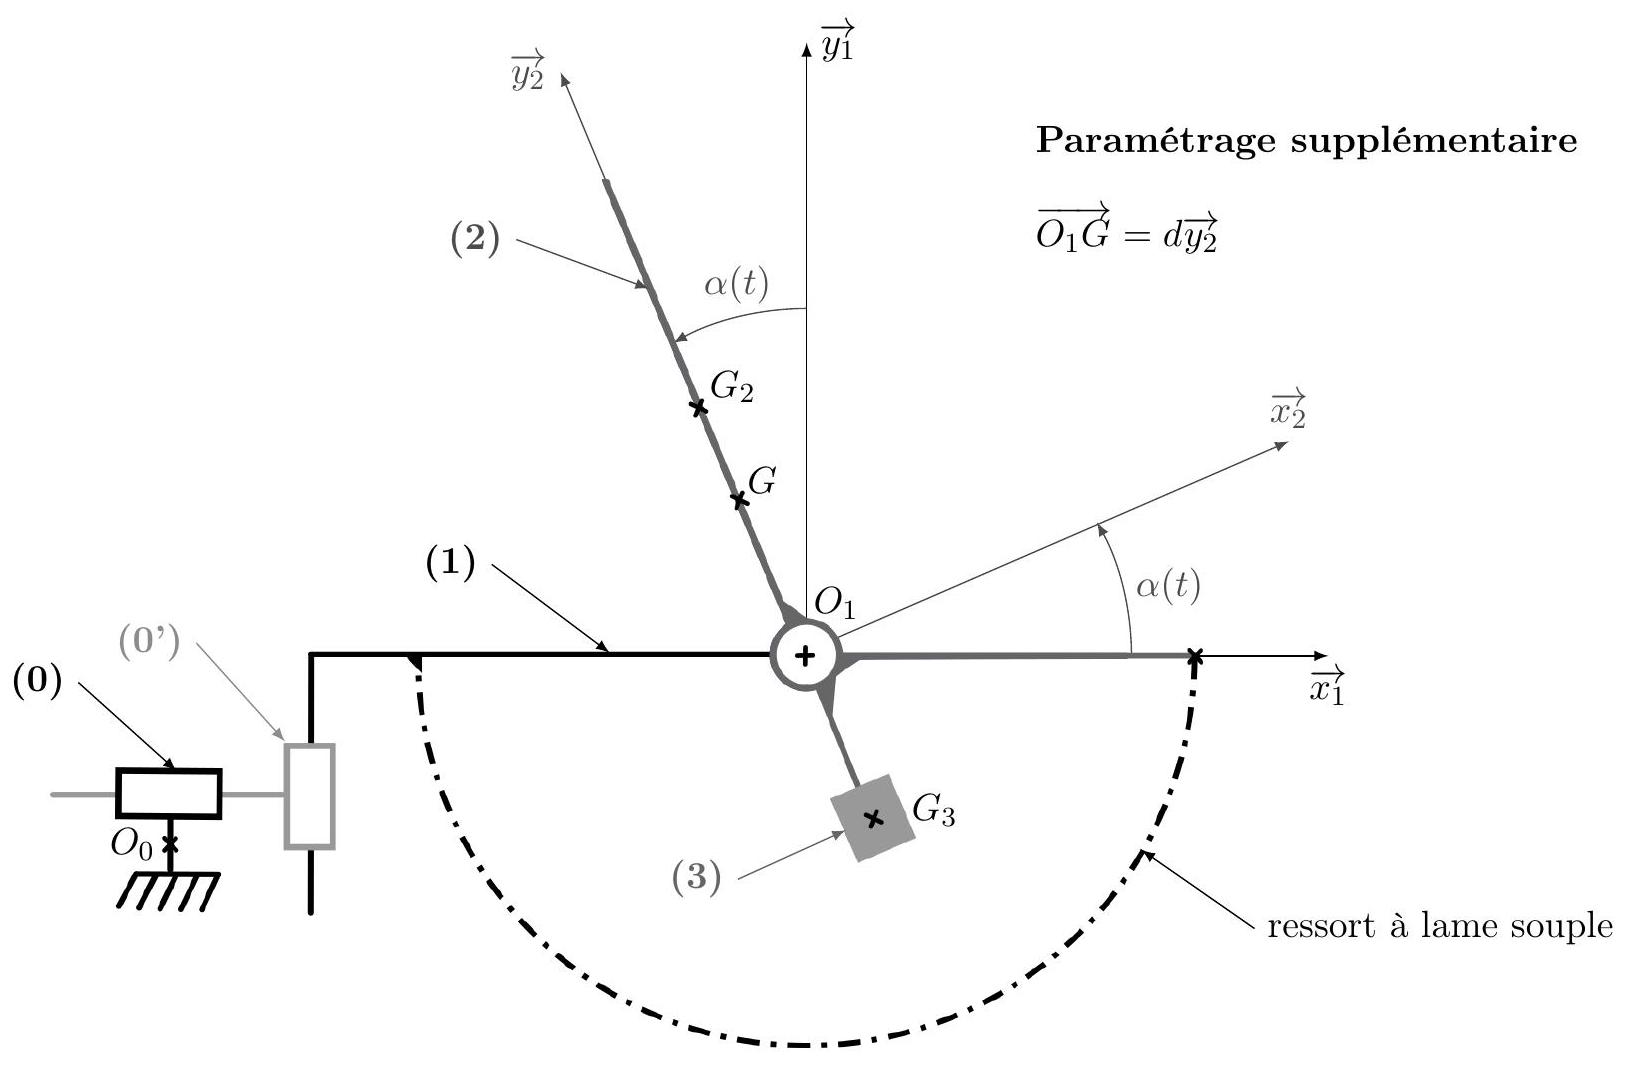
\includegraphics[max width=\textwidth]{2024_04_26_3285cfc264024262add0g-18}
\end{center}

Notations et hypothèses supplémentaires

\begin{center}
\begin{tabular}{|c|l|}
\hline
$G$ & \begin{tabular}{l}
centre d'inertie de l'ensemble mobile \\
$\{(\mathbf{2})+(\mathbf{3})\}$ testé sur Terre \\
\end{tabular} \\
\hline
$M$ & masse de l'ensemble mobile $\{\mathbf{( 2 )}+\mathbf{( 3 )}\}$ \\
\hline
$I_{z z}$ & \begin{tabular}{l}
moment d'inertie de l'ensemble mobile \\
$\{(\mathbf{2})+(\mathbf{3})\}$ sur l'axe $\left(O_{1}, \overrightarrow{z_{1}}\right)$ \\
\end{tabular} \\
\hline
\end{tabular}
\end{center}

Le référentiel $\mathcal{R}_{0}$, auquel est associé le repère $R_{0}=\left(O_{0}, \overrightarrow{x_{1}}, \overrightarrow{y_{1}}, \overrightarrow{z_{1}}\right)$, est supposé galiléen.

On note la vitesse du sol (1) par rapport à $R_{0}$ :

$$
\vec{V}_{\left(O_{1}, 1 / R_{0}\right)}=V_{x}(t) \overrightarrow{x_{1}}+V_{y}(t) \overrightarrow{y_{1}}
$$

Grâce au contrepoids, l'action de la pesanteur sur l'ensemble mobile qui s'applique en $G$ a un moment en $O_{1}$ égal à celui que subirait le pendule seul sur Mars :

$\left\{\mathcal{T}_{\text {pesanteur } \rightarrow(2+3)}\right\}=\left\{\begin{array}{c}-\left(M_{2}+m_{3}\right) g_{\mathrm{T}} \overrightarrow{y_{1}} \\ a M_{2} g_{M} \sin \alpha(t) \overrightarrow{z_{1}}\end{array}\right\}_{O_{1}}$

Aucune autre action de pesanteur n'est à prendre en compte.

Le système de réglage de la position du centre d'inertie $G_{2}$ permet d'imposer $\alpha_{\text {eq }}=\alpha_{0}$. Dans ces conditions, l'équation traduisant l'équilibre de l'ensemble mobile en l'absence de séisme reste valable et se simplifie ainsi :


\begin{equation*}
a M_{2} g_{\mathrm{M}} \sin \alpha_{0}+C_{0}=0 \tag{eq.1'}
\end{equation*}


\section*{Annexe 5 - Asservissement en tension d'un système}
Schéma-blocs de l'asservissement

\begin{center}
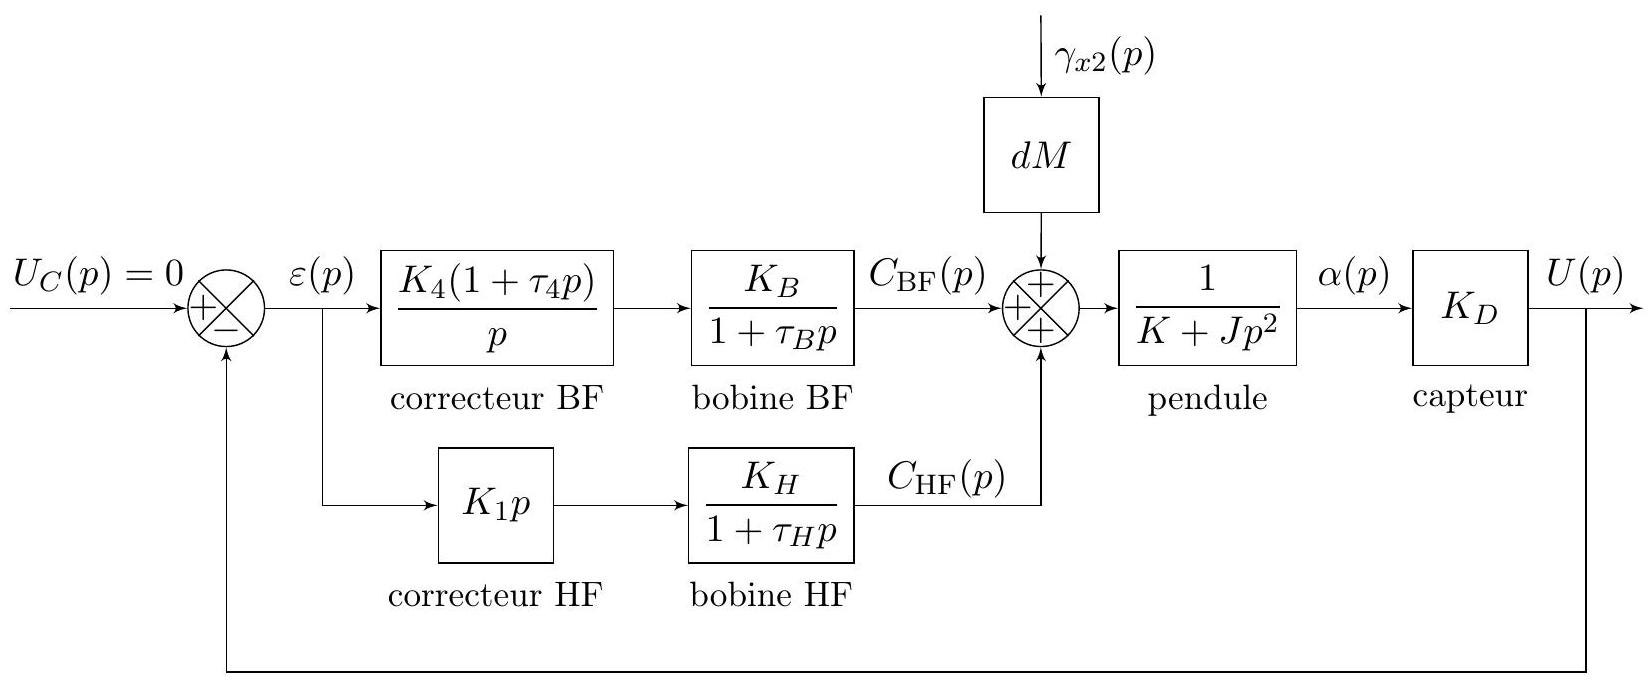
\includegraphics[max width=\textwidth]{2024_04_26_3285cfc264024262add0g-19}
\end{center}

Grandeurs physiques intervenant dans l'asservissement

\begin{center}
\begin{tabular}{|c|c|c|l|}
\hline
\begin{tabular}{c}
Grandeur \\
physique \\
\end{tabular} & \begin{tabular}{c}
Transformée \\
de Laplace \\
\end{tabular} & Unité & Description \\
\hline\hline
$u_{C}(t)$ & $U_{C}(p)$ & $\mathrm{V}$ & \begin{tabular}{l}
Tension consigne. Elle est toujours nulle car on souhaite que le \\
pendule revienne à sa position d'équilibre. \\
\end{tabular} \\
\hline
$u(t)$ & $U(p)$ & $\mathrm{V}$ & \begin{tabular}{l}
Tension en sortie du capteur, image du déplacement angulaire \\
du pendule autour de sa position d'équilibre \\
\end{tabular} \\
\hline
$\varepsilon(t)$ & $\varepsilon(p)$ & $\mathrm{V}$ & \begin{tabular}{l}
Écart entre la tension de consigne et la tension en sortie du \\
capteur \\
\end{tabular} \\
\hline
$\gamma_{x 2}(t)$ & $\gamma_{x 2}(p)$ & $\mathrm{m} \cdot \mathrm{s}^{-2}$ & Accélération du sol lors d'un séisme \\
\hline
$\Delta \alpha(t)$ & $\alpha(p)$ & $\mathrm{rad}$ & \begin{tabular}{l}
Déplacement angulaire du pendule autour de sa position d'équi- \\
libre \\
\end{tabular} \\
\hline
$C_{\mathrm{BF}}(t)$ & $C_{\mathrm{BF}}(p)$ & $\mathrm{N} \cdot \mathrm{m}$ & Moment généré par la bobine BF sur l'axe de rotation du pendule \\
\hline
$C_{\mathrm{HF}}(t)$ & $C_{\mathrm{HF}}(p)$ & $\mathrm{N} \cdot \mathrm{m}$ & Moment généré par la bobine HF sur l'axe de rotation du pendule \\
\hline
\end{tabular}
\end{center}

\section*{Données numériques}
\begin{itemize}
  \item $K_{D}=1,48 \times 10^{5} \mathrm{~V} \cdot \mathrm{rad}^{-1}$
  \item $K_{H}=3 \times 10^{-8} \mathrm{~N} \cdot \mathrm{m} \cdot \mathrm{V}^{-1}$
  \item $\tau_{H}=0,001 \mathrm{~s}$
  \item $K_{B}=5 \times 10^{-8} \mathrm{~N} \cdot \mathrm{m} \cdot \mathrm{V}^{-1}$
  \item $\tau_{B}=0,1 \mathrm{~s}$
\end{itemize}

\begin{center}
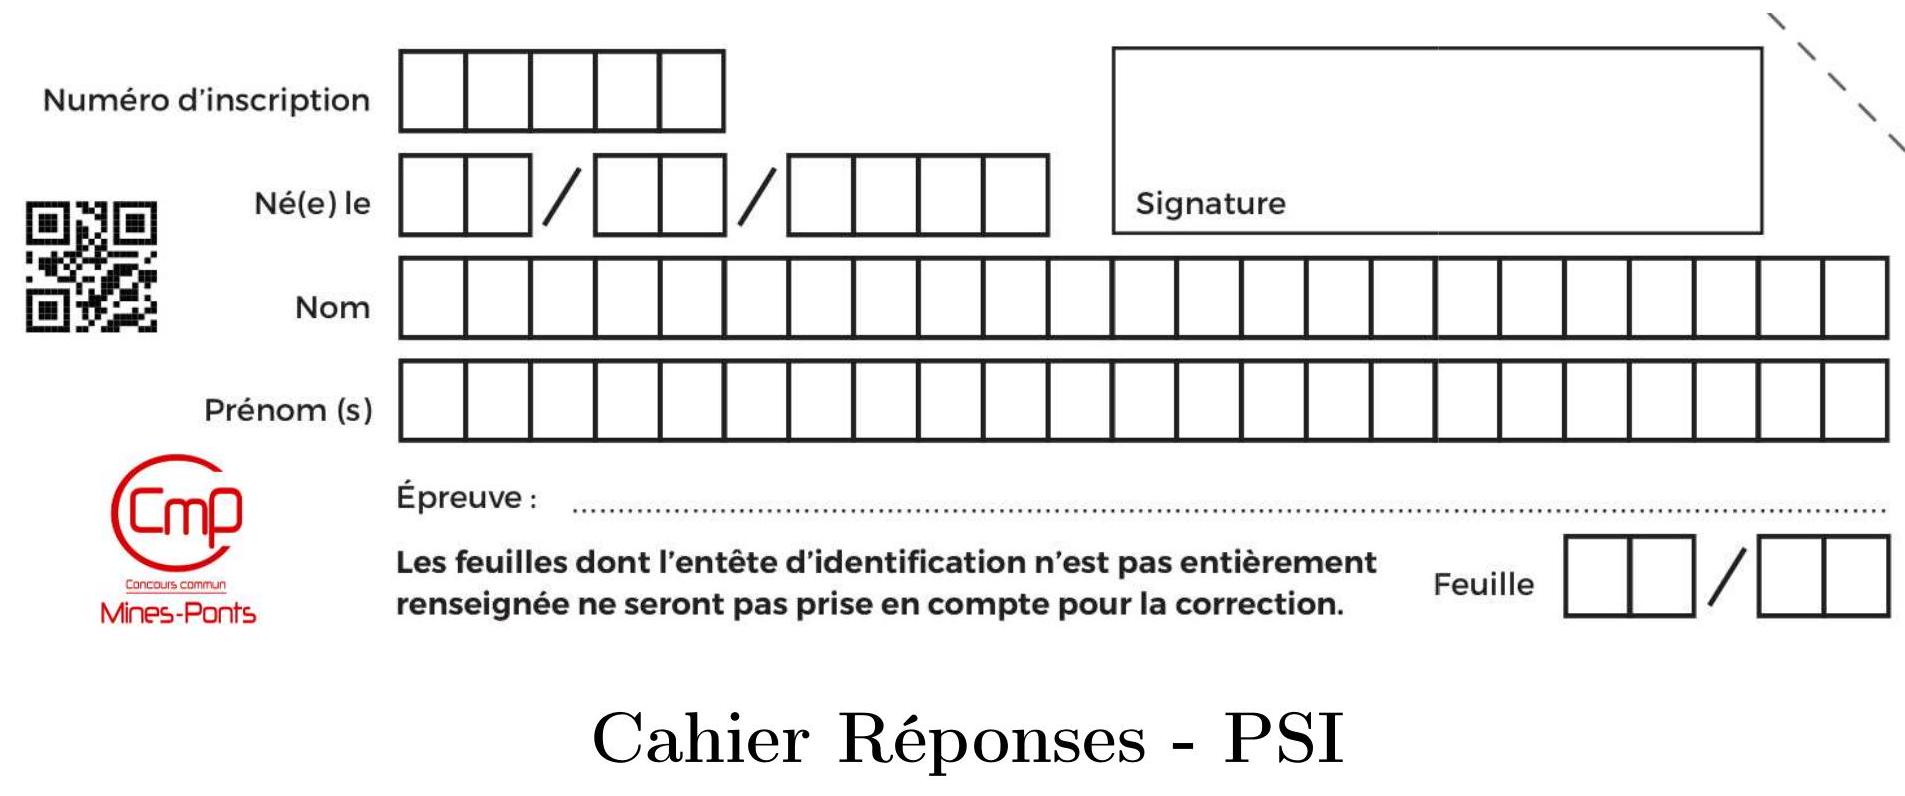
\includegraphics[max width=\textwidth]{2024_04_26_3285cfc264024262add0g-20}
\end{center}

Question 1 Bilan des Actions Mécaniques Extérieures:

Théorème ou Principe utilisé, éléments d'application :

Équation d'équilibre :

\begin{center}
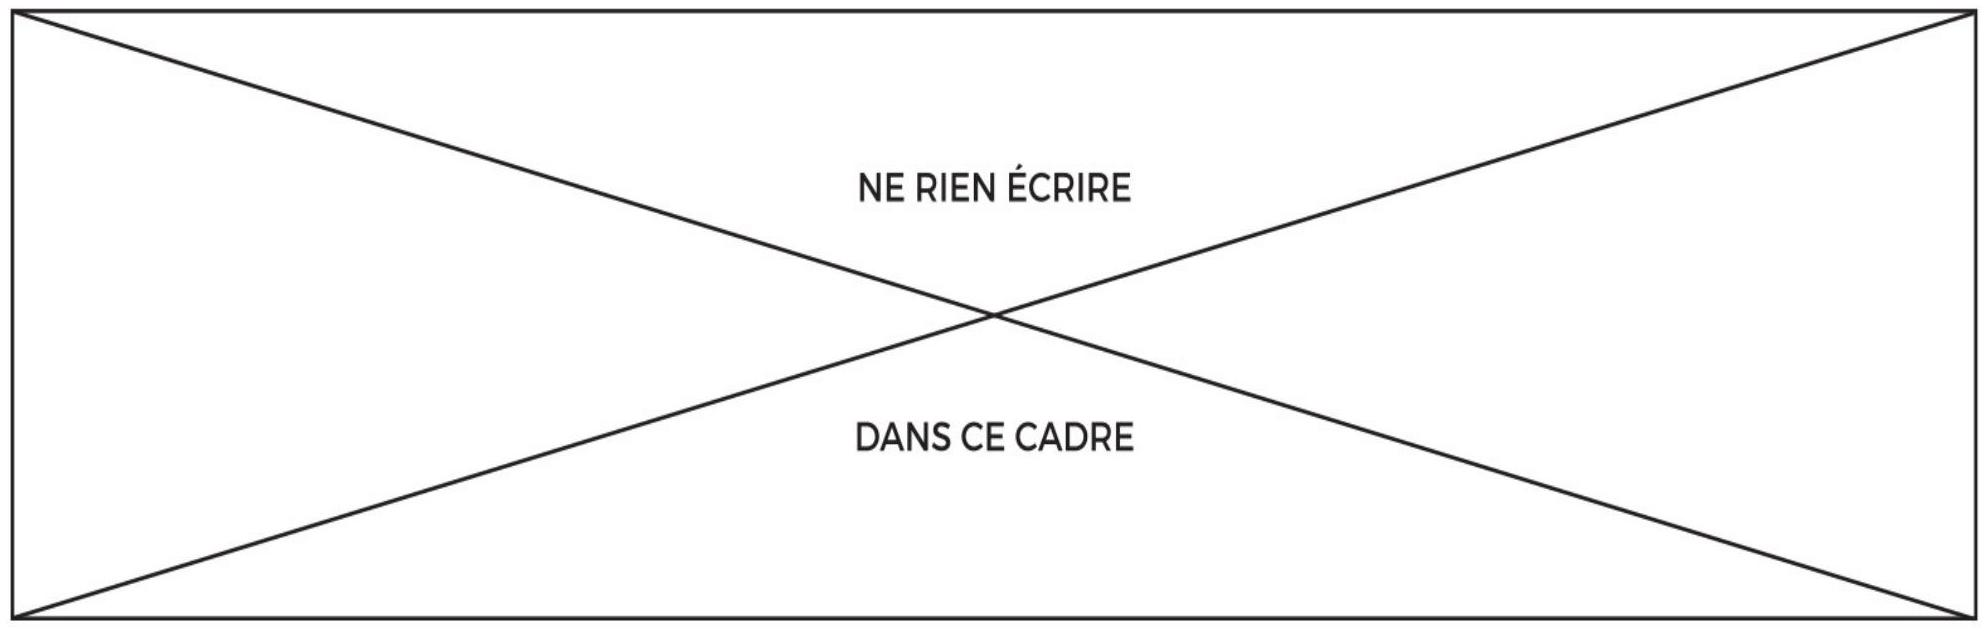
\includegraphics[max width=\textwidth]{2024_04_26_3285cfc264024262add0g-21}
\end{center}

Question 2

$$
b m_{3}=
$$

Question 3

顷(2)

(4)

\section*{Question 4}
$m_{i}=$

$m_{u}=$

$$
h=
$$

Intérêt de l'hyperstatisme :

\section*{Question 5}
Liaison $(\mathrm{N}) /(5)$ :

Justification :

Liaison $(\mathrm{N}) /(\mathrm{v})$ :

Justification :

\section*{Question 6}
\begin{center}
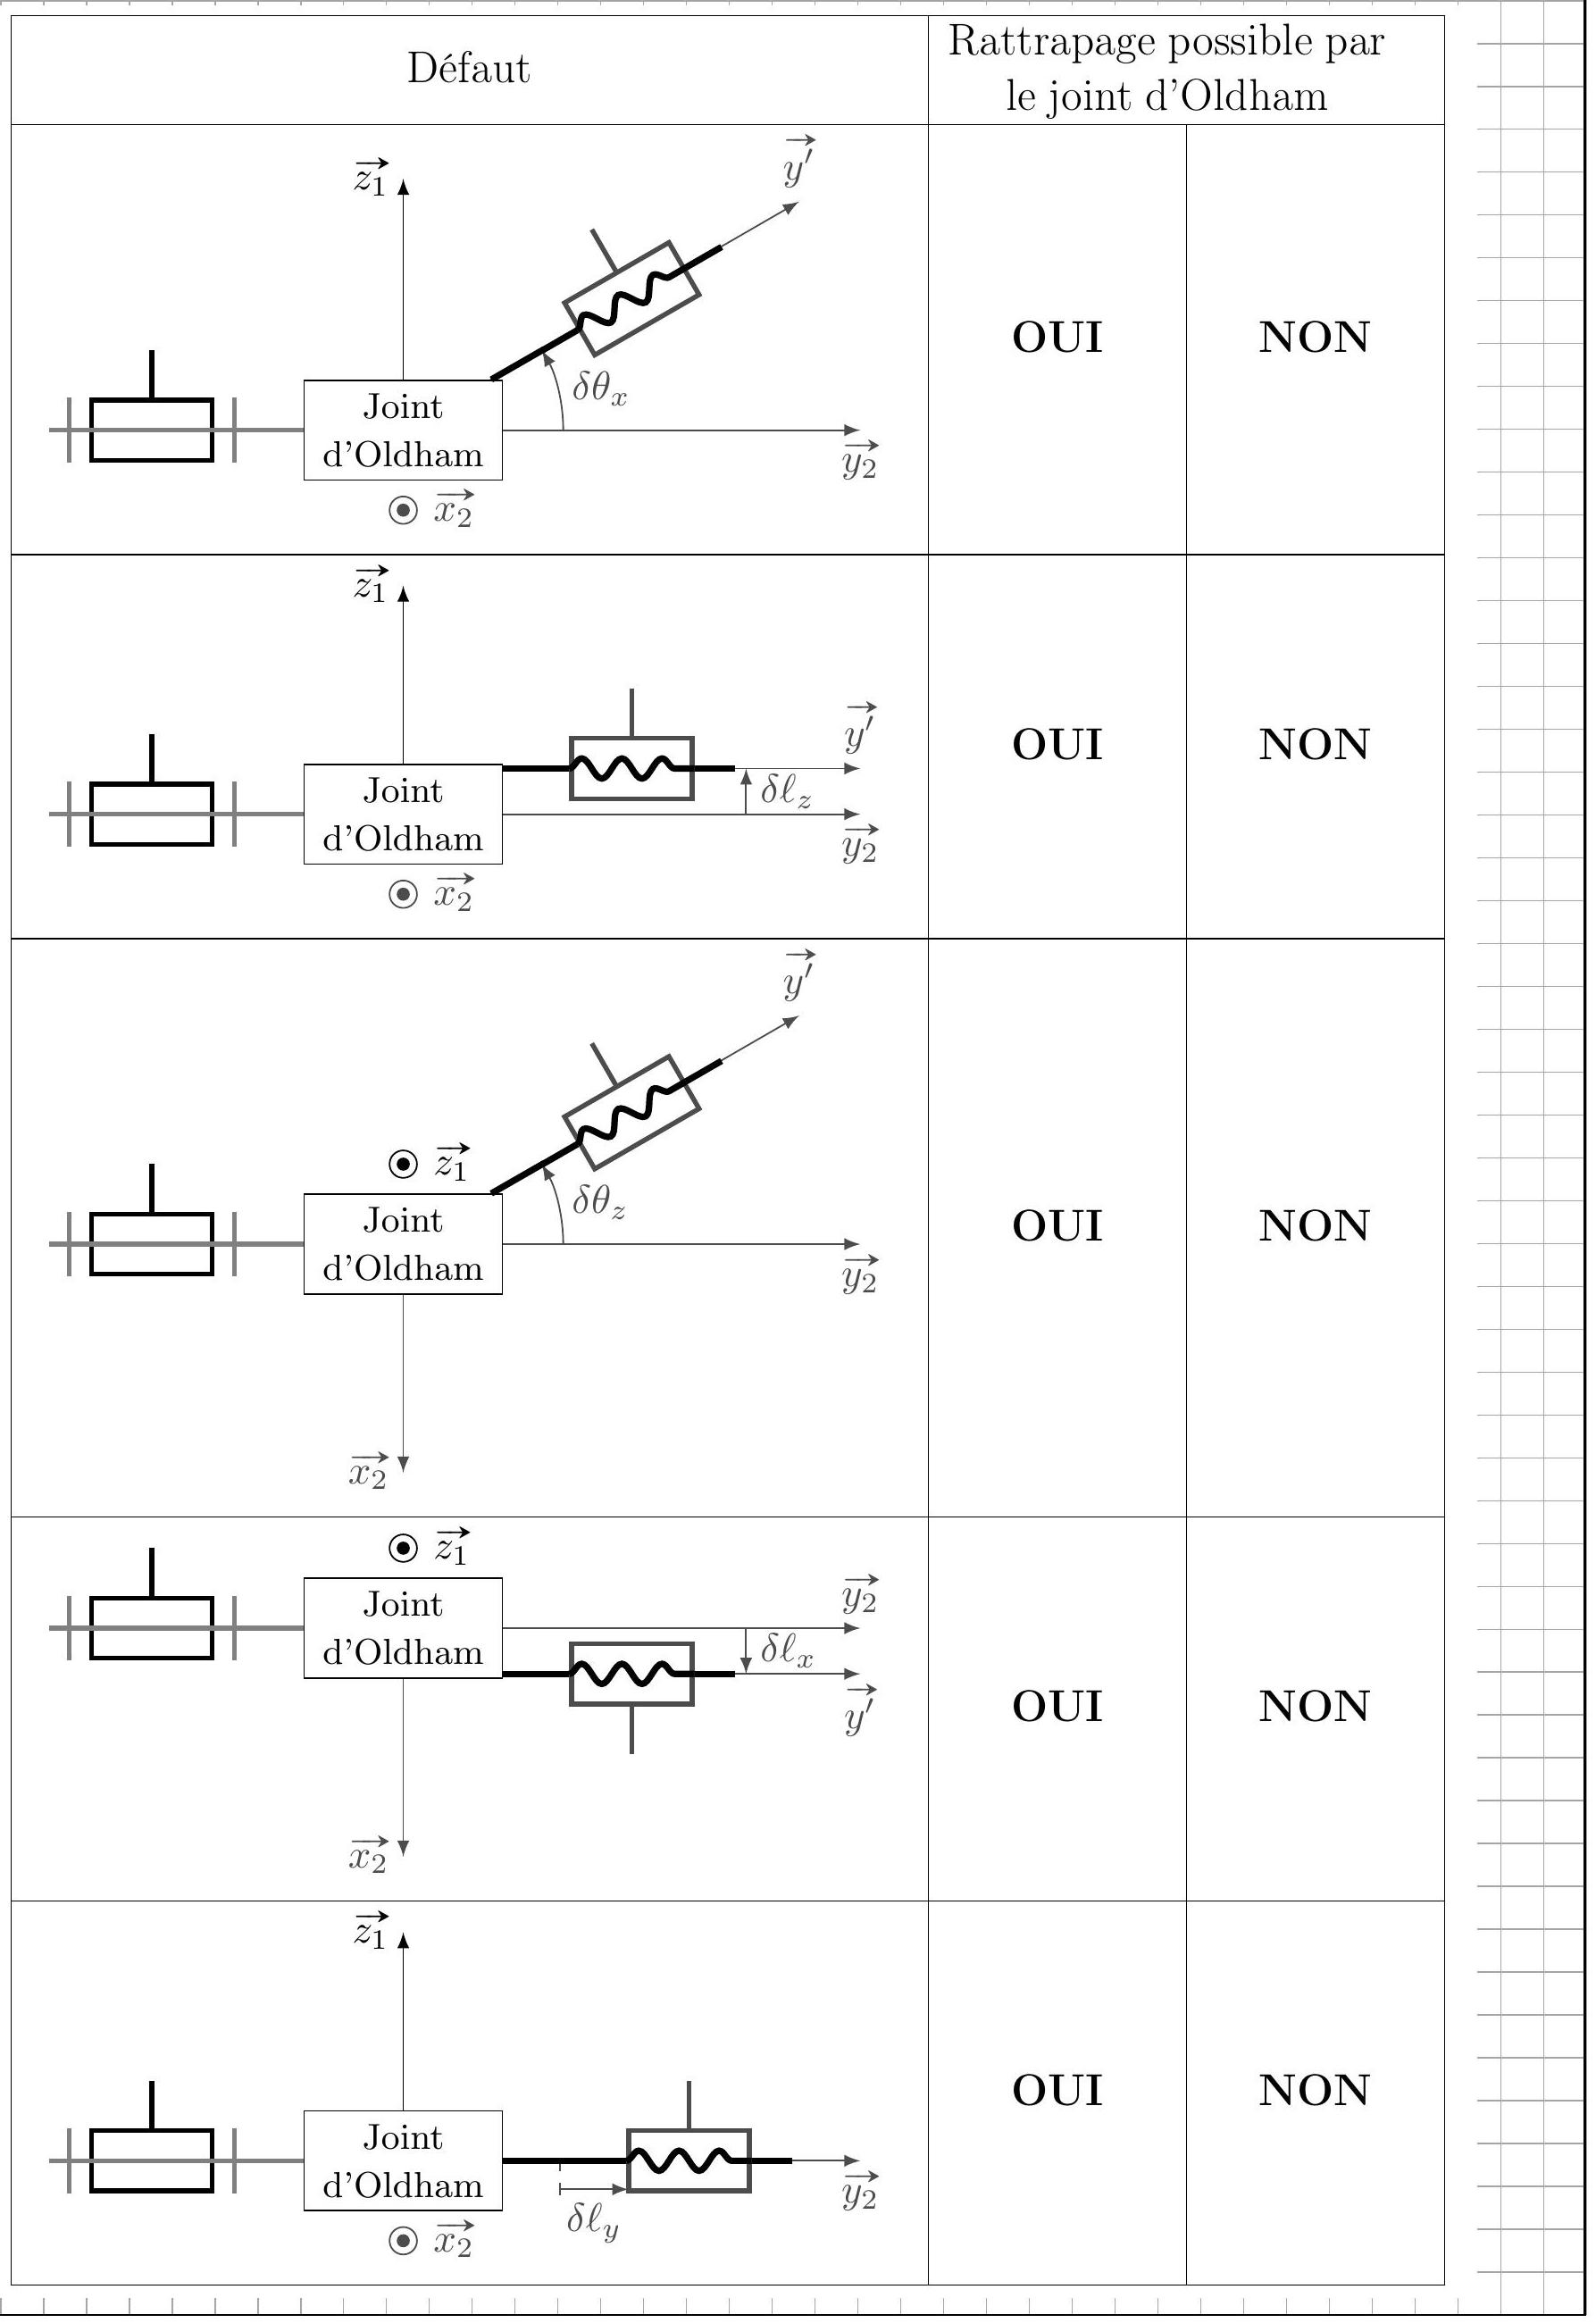
\includegraphics[max width=\textwidth]{2024_04_26_3285cfc264024262add0g-23}
\end{center}

\begin{center}
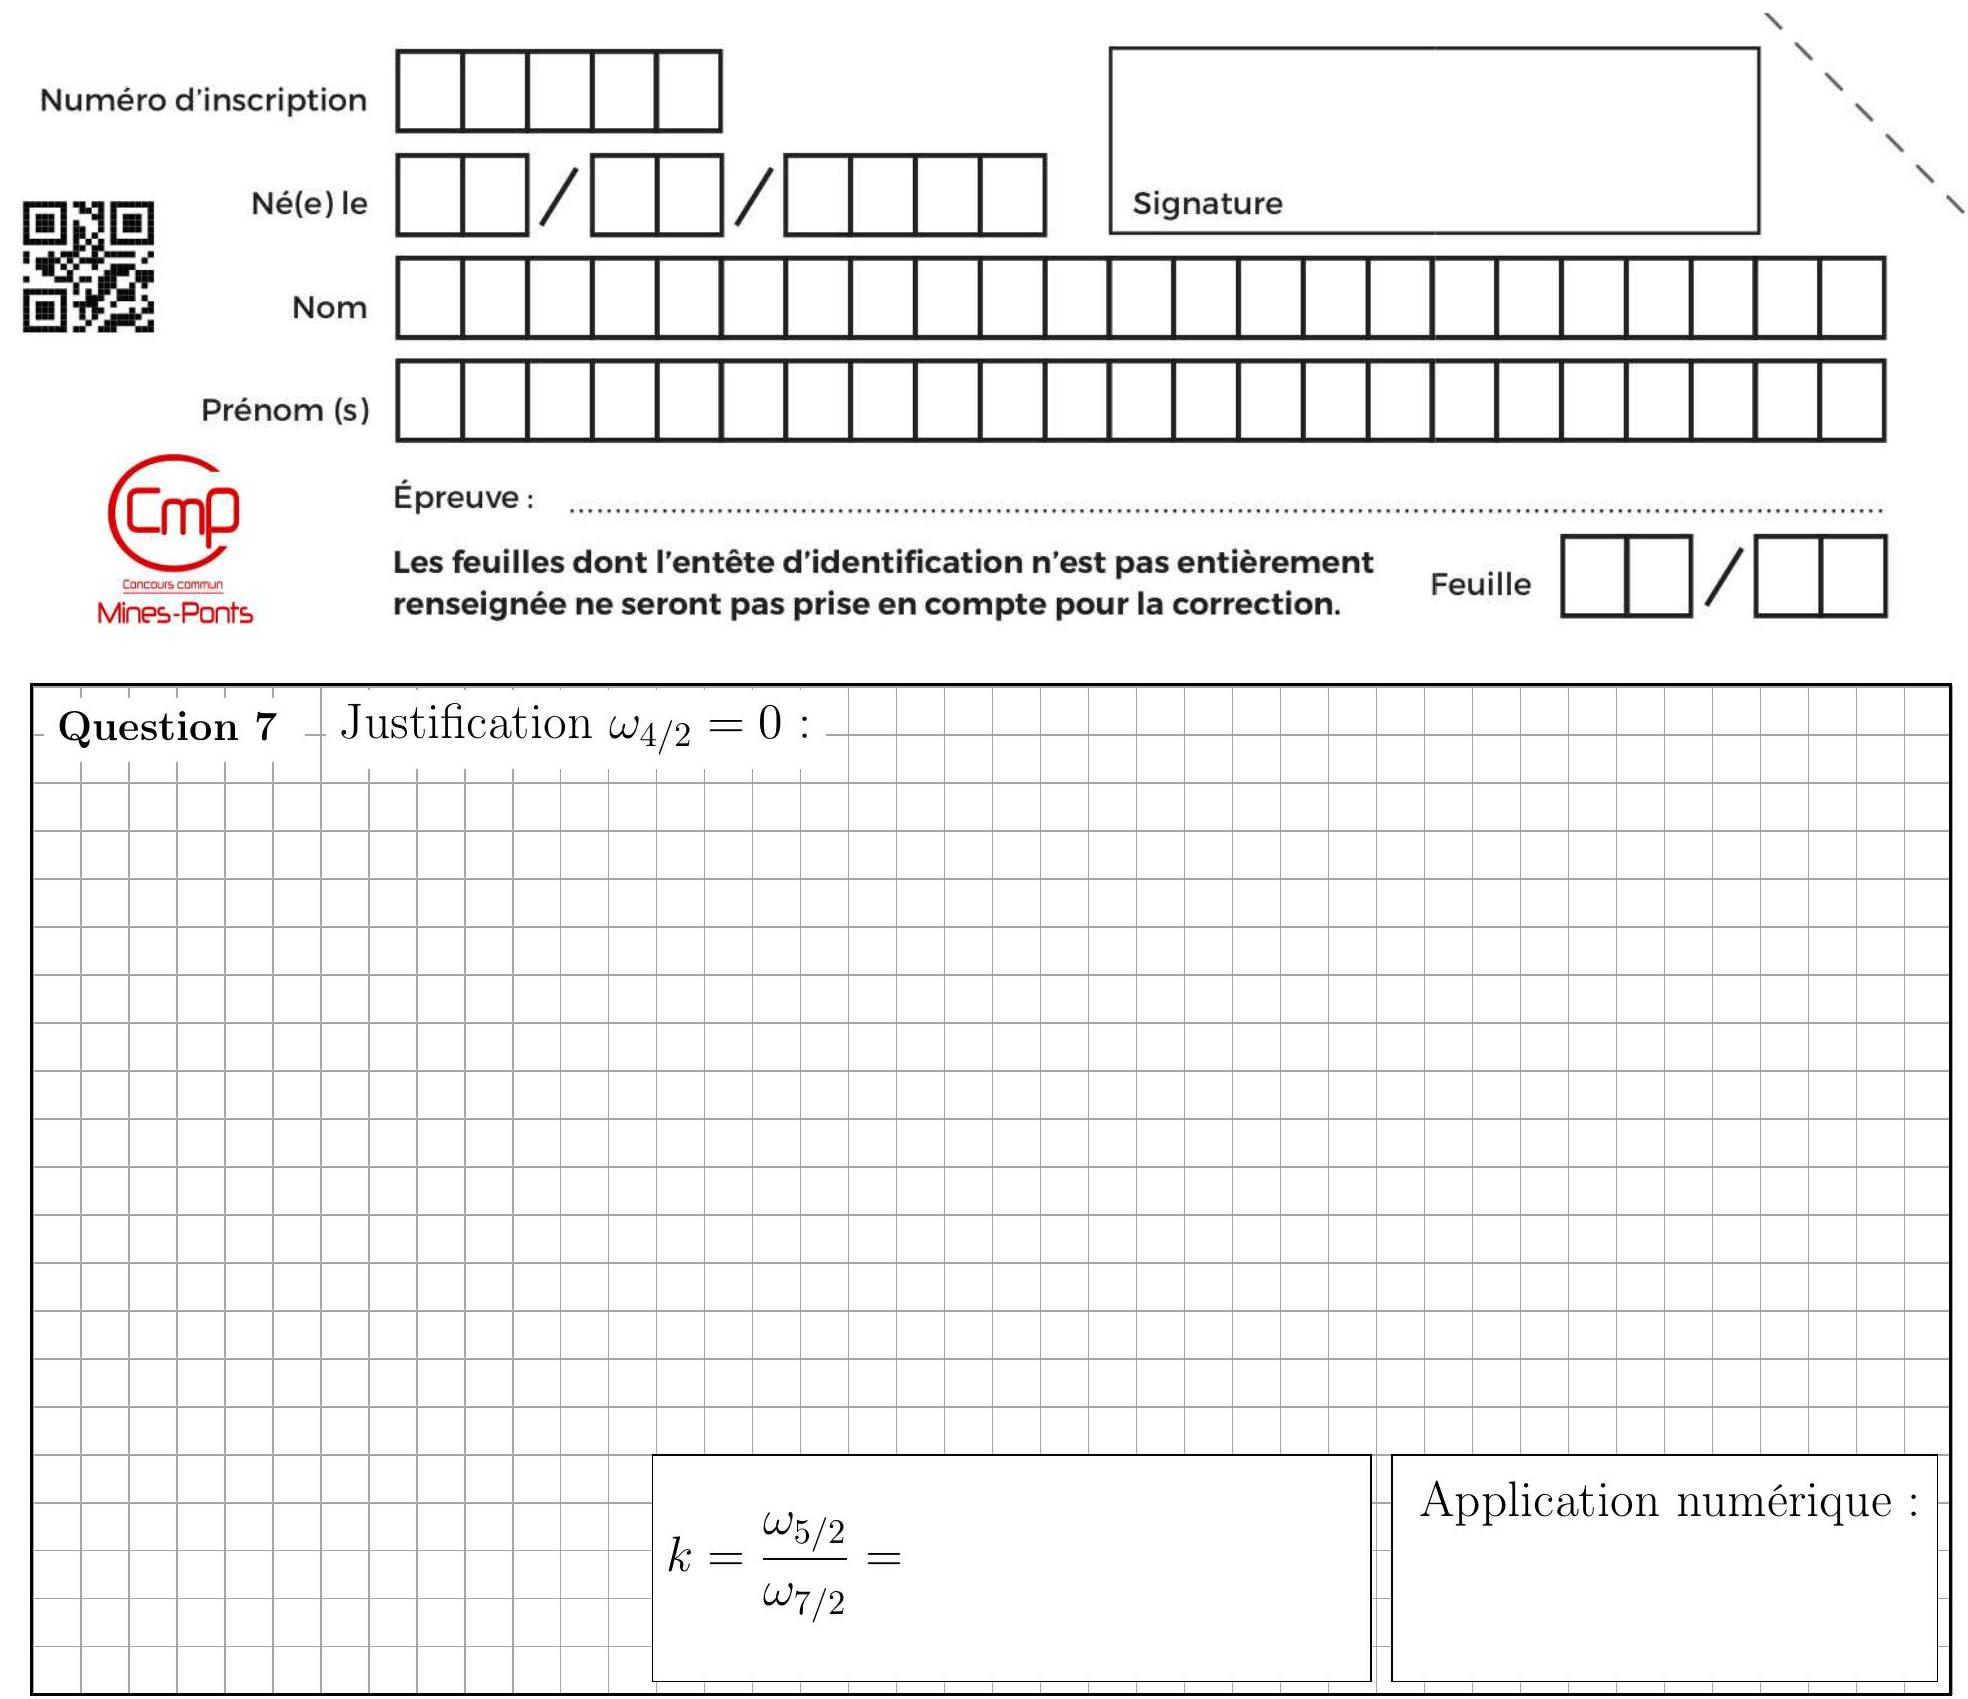
\includegraphics[max width=\textwidth]{2024_04_26_3285cfc264024262add0g-24}
\end{center}

\section*{Question 8}
$$
k_{g}=\frac{\omega_{5 / 2}}{\omega_{m / 2}}=
$$

\section*{Question 9}
$d_{v}=$

Application numérique : $d_{v}=$

Conclusion vis-à-vis de l'exigence 1.1 :

\begin{center}
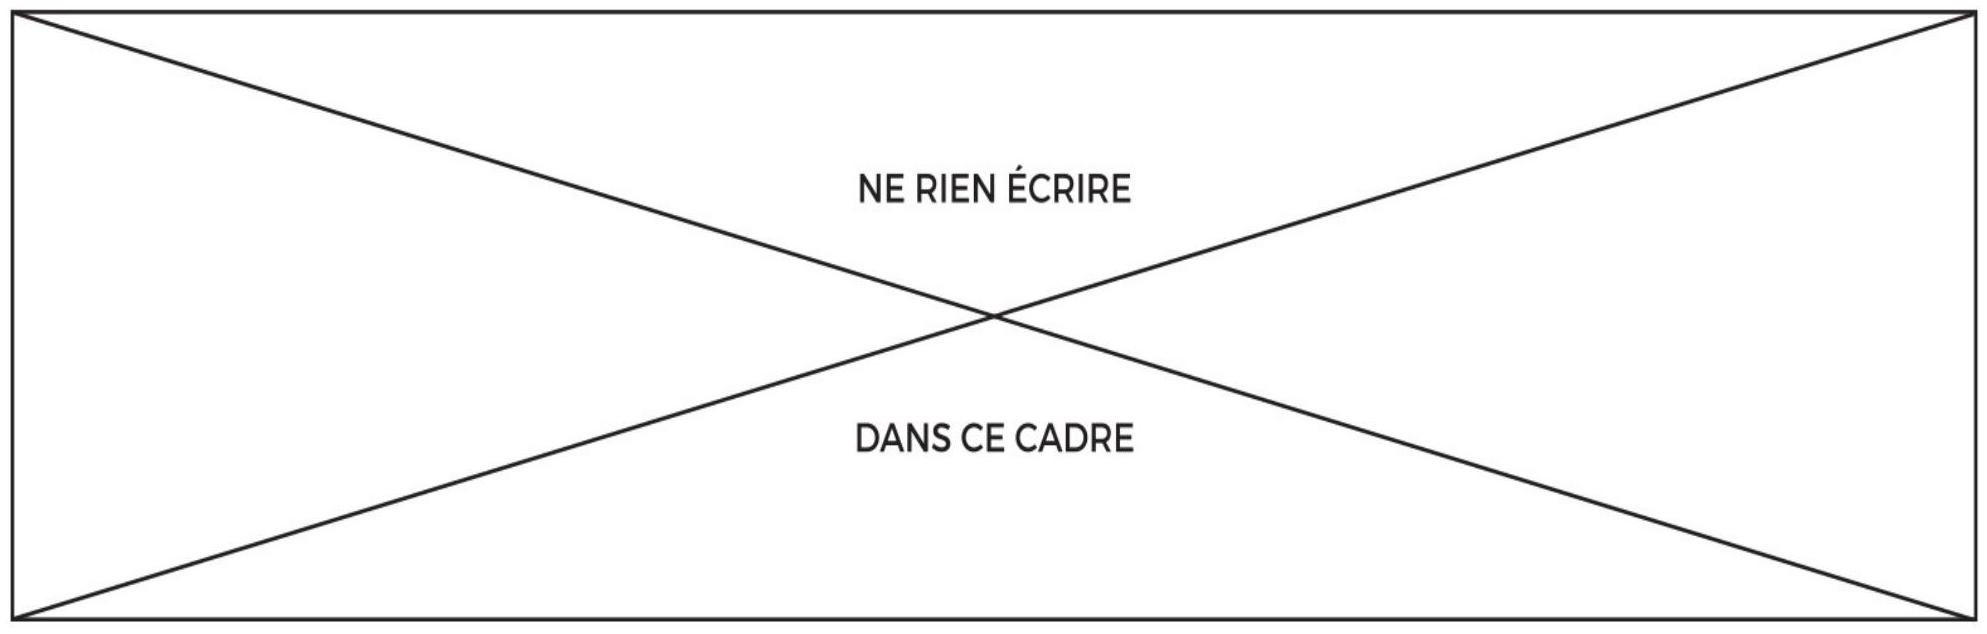
\includegraphics[max width=\textwidth]{2024_04_26_3285cfc264024262add0g-25}
\end{center}

Question 10

Question 11

Erreur de positionnement :

Conclusion vis-à-vis de l'exigence 1.1:

Question 12 - Plan de symétrie:

$$
\overline{\bar{I}}_{\left(O_{1}, 2+3\right)}=
$$

Question 13

$\vec{\sigma}_{O_{1},(2+3) / R_{0}}=$

Question 14 Calcul de $\vec{\delta}_{O_{1},(2+3) / R_{0}} \cdot \overrightarrow{z_{1}}$ :

$$
\gamma_{x 2}(t)=
$$

\section*{Question 15}
Système isolé :

Théorème utilisé :

Justification équation non-linéaire :

Question 16

\begin{center}
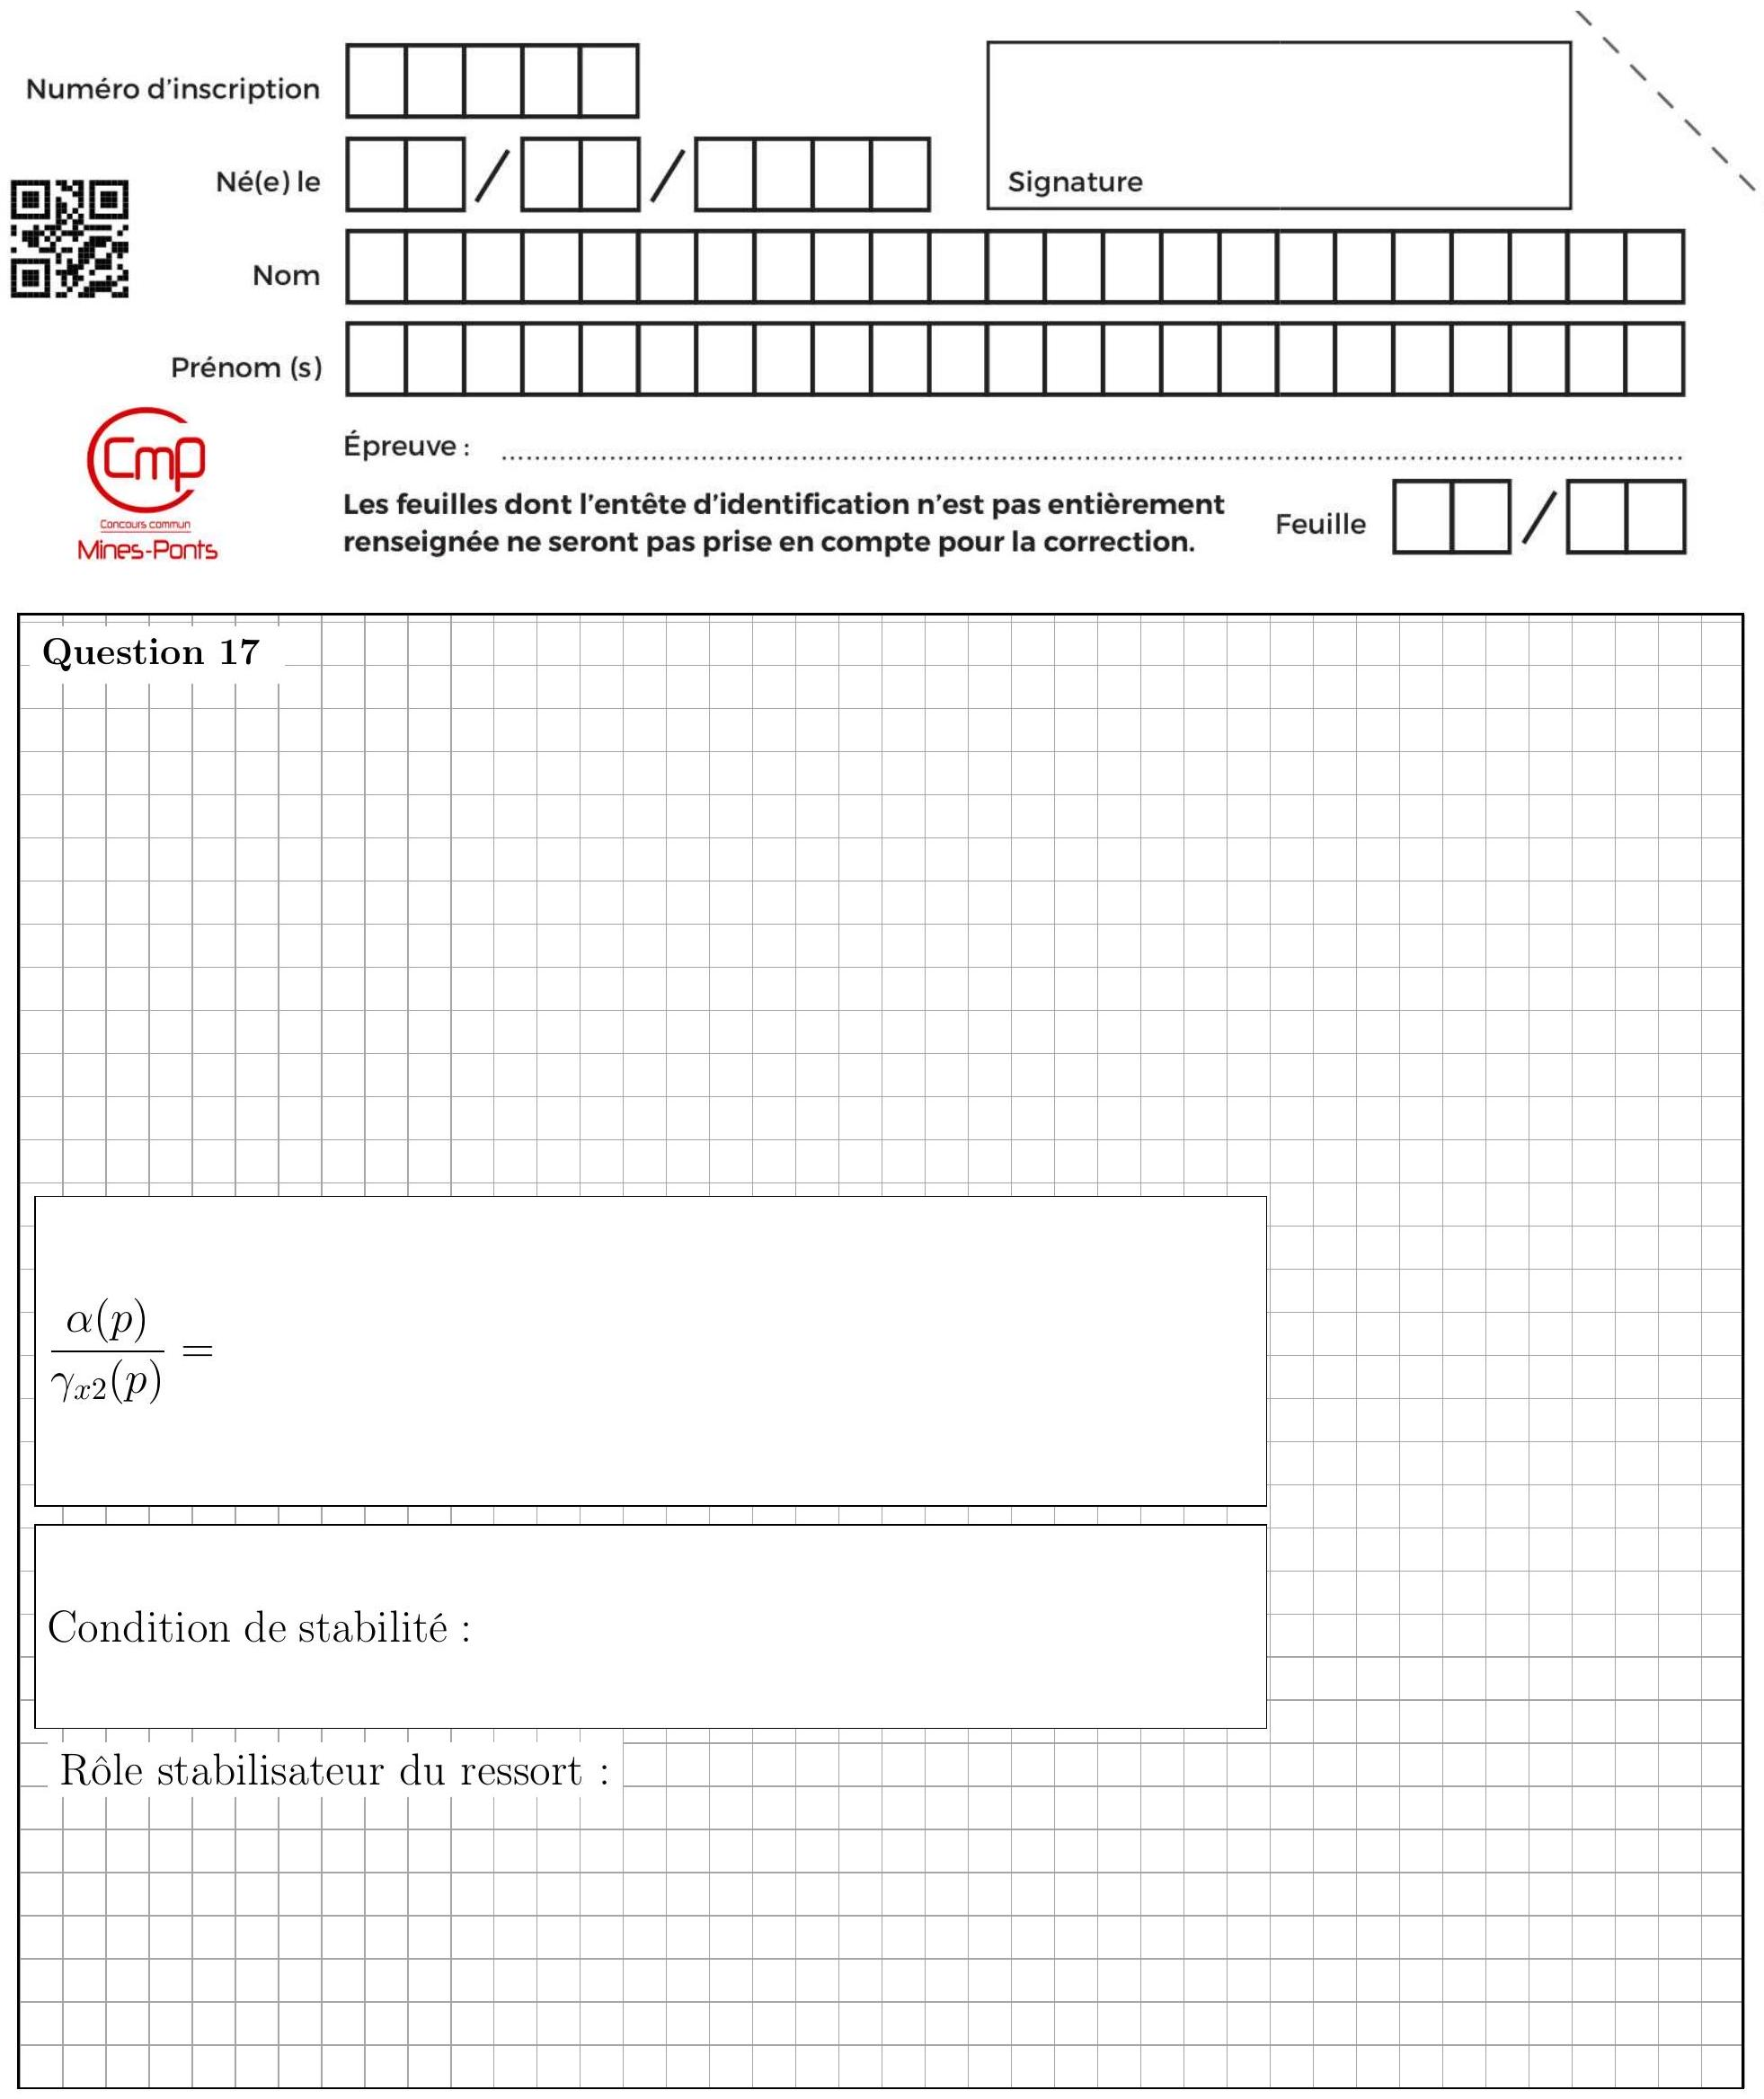
\includegraphics[max width=\textwidth]{2024_04_26_3285cfc264024262add0g-28}
\end{center}

\section*{Question 18}
$A=\quad \omega_{0}=\quad \xi=$

\begin{center}
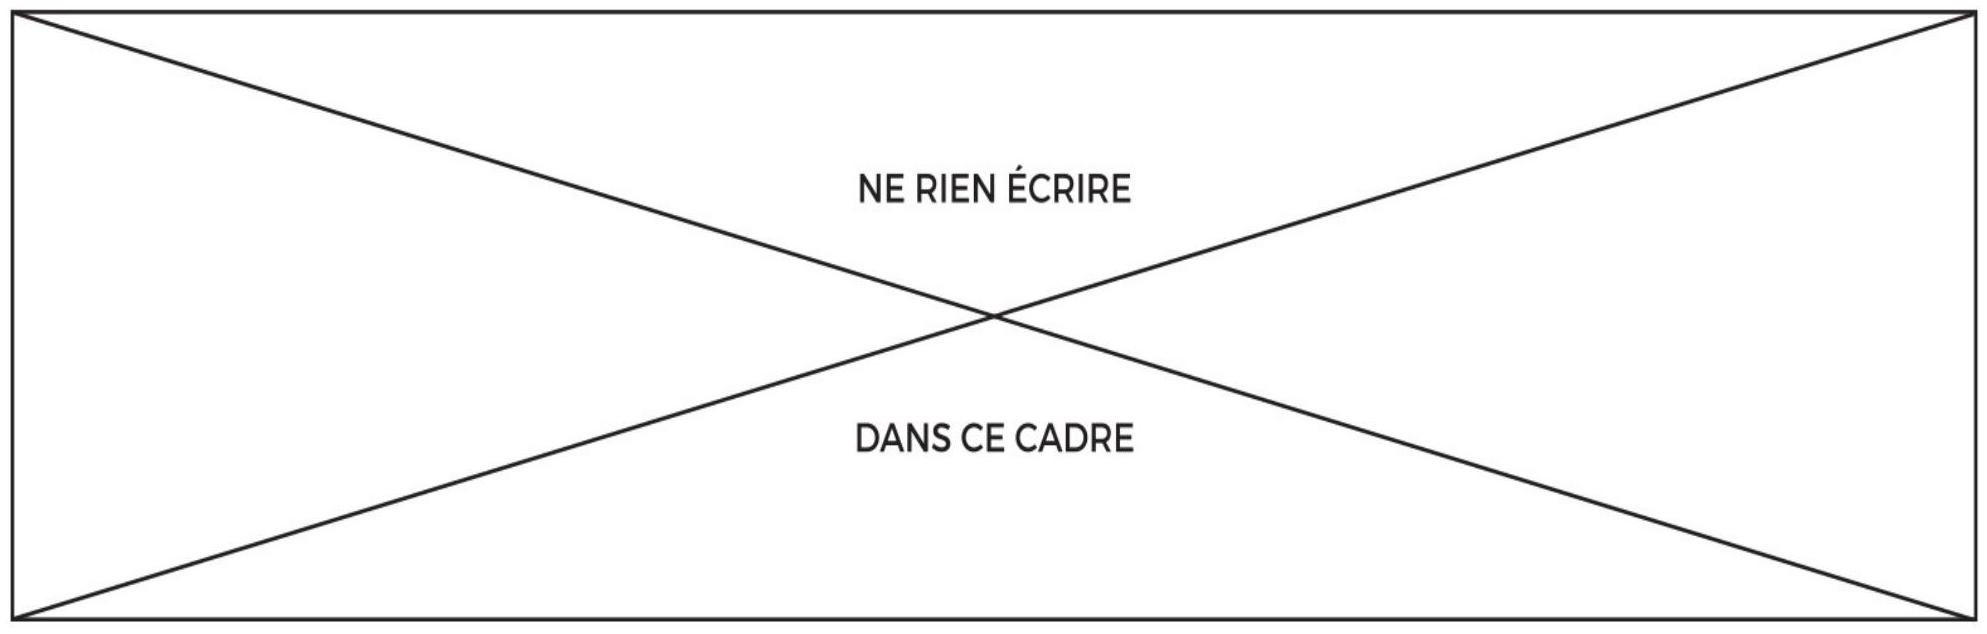
\includegraphics[max width=\textwidth]{2024_04_26_3285cfc264024262add0g-29}
\end{center}

Question 19

$C_{0}=$

Question 20

Plage de valeurs de $k$ :

Question 21

\begin{center}
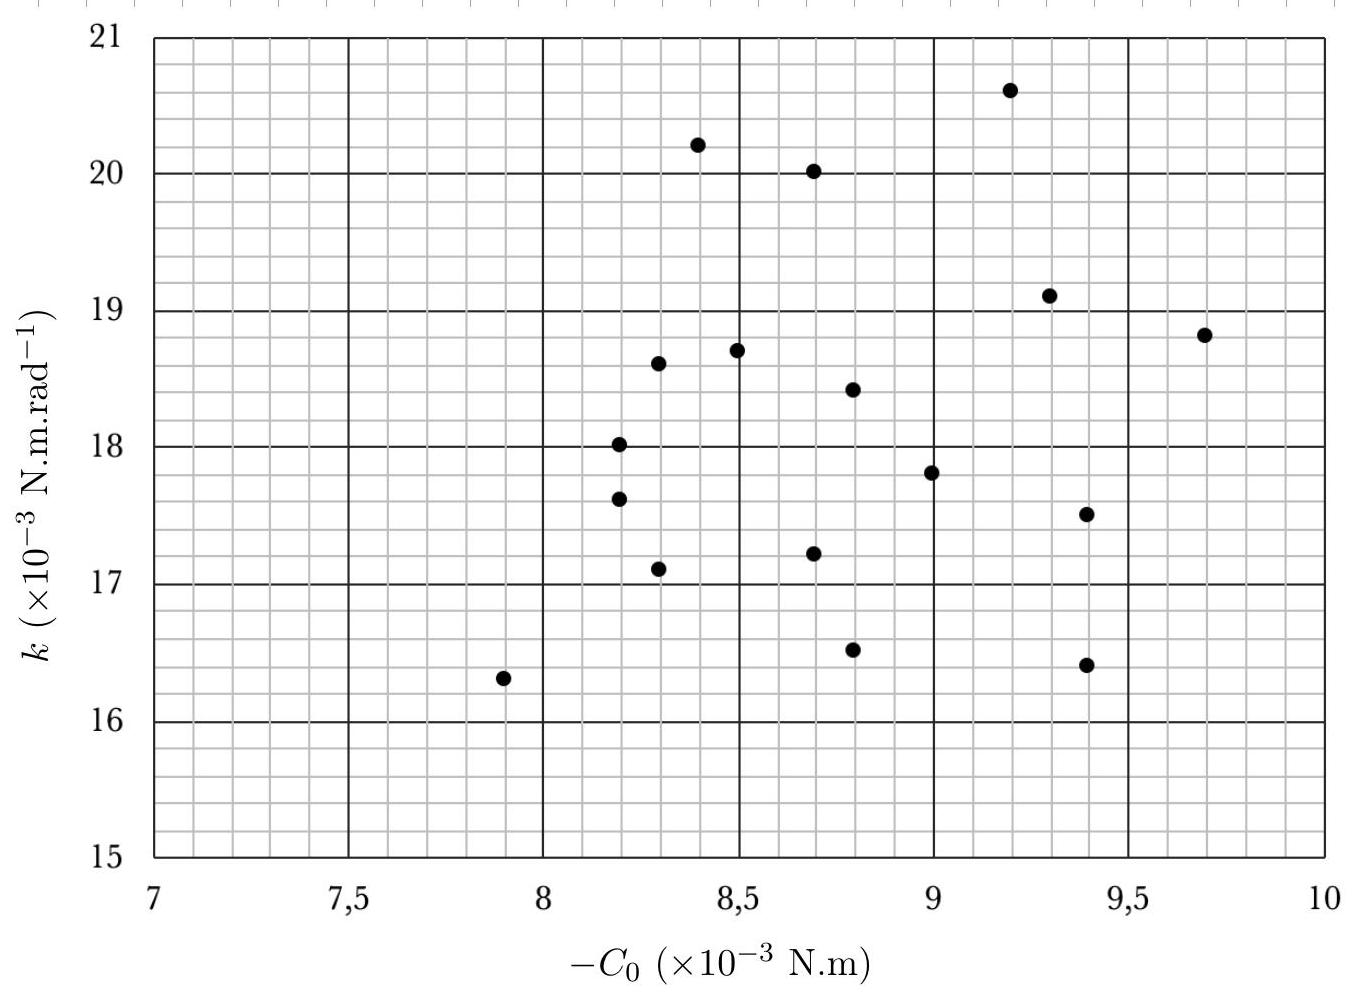
\includegraphics[max width=\textwidth]{2024_04_26_3285cfc264024262add0g-30}
\end{center}

Figure A

\section*{Question 22}
\begin{center}
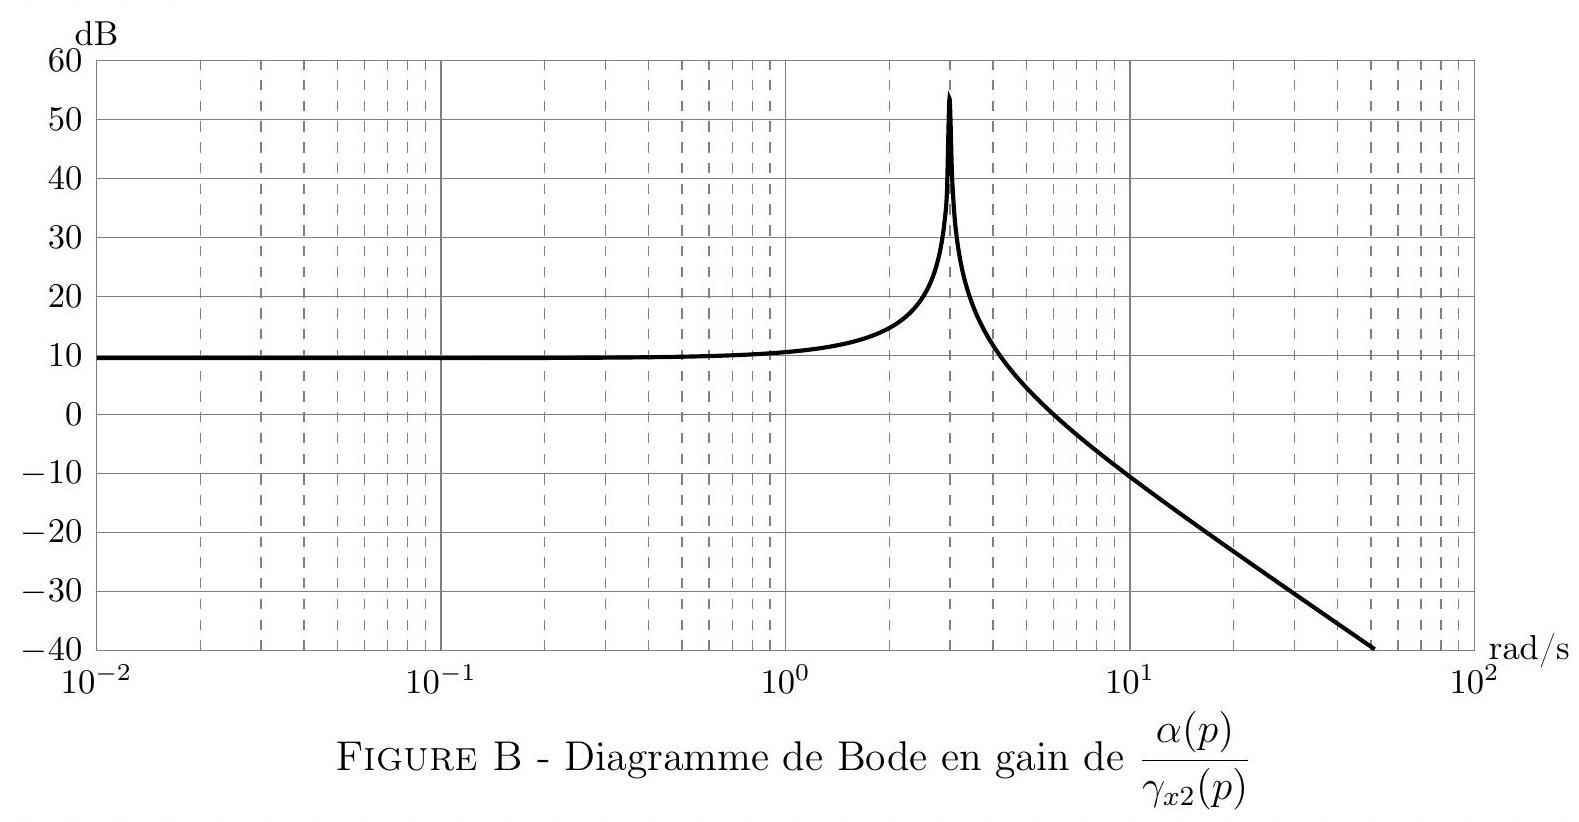
\includegraphics[max width=\textwidth]{2024_04_26_3285cfc264024262add0g-30(1)}
\end{center}

Conclusion :

Question 23

\begin{center}
\begin{tabular}{|l|l|}
\hline
$H_{\gamma}(p)=$ \\
\hline
$k_{\mathrm{HF}}=$ \\
\hline
$b_{1}=$ \\
\hline
$b_{2}=$ \\
\hline
$a_{1}=$ \\
\hline
$b_{3}=$ \\
\hline
\end{tabular}
\end{center}

Question 24 - Justification de la stabilité :

\begin{center}
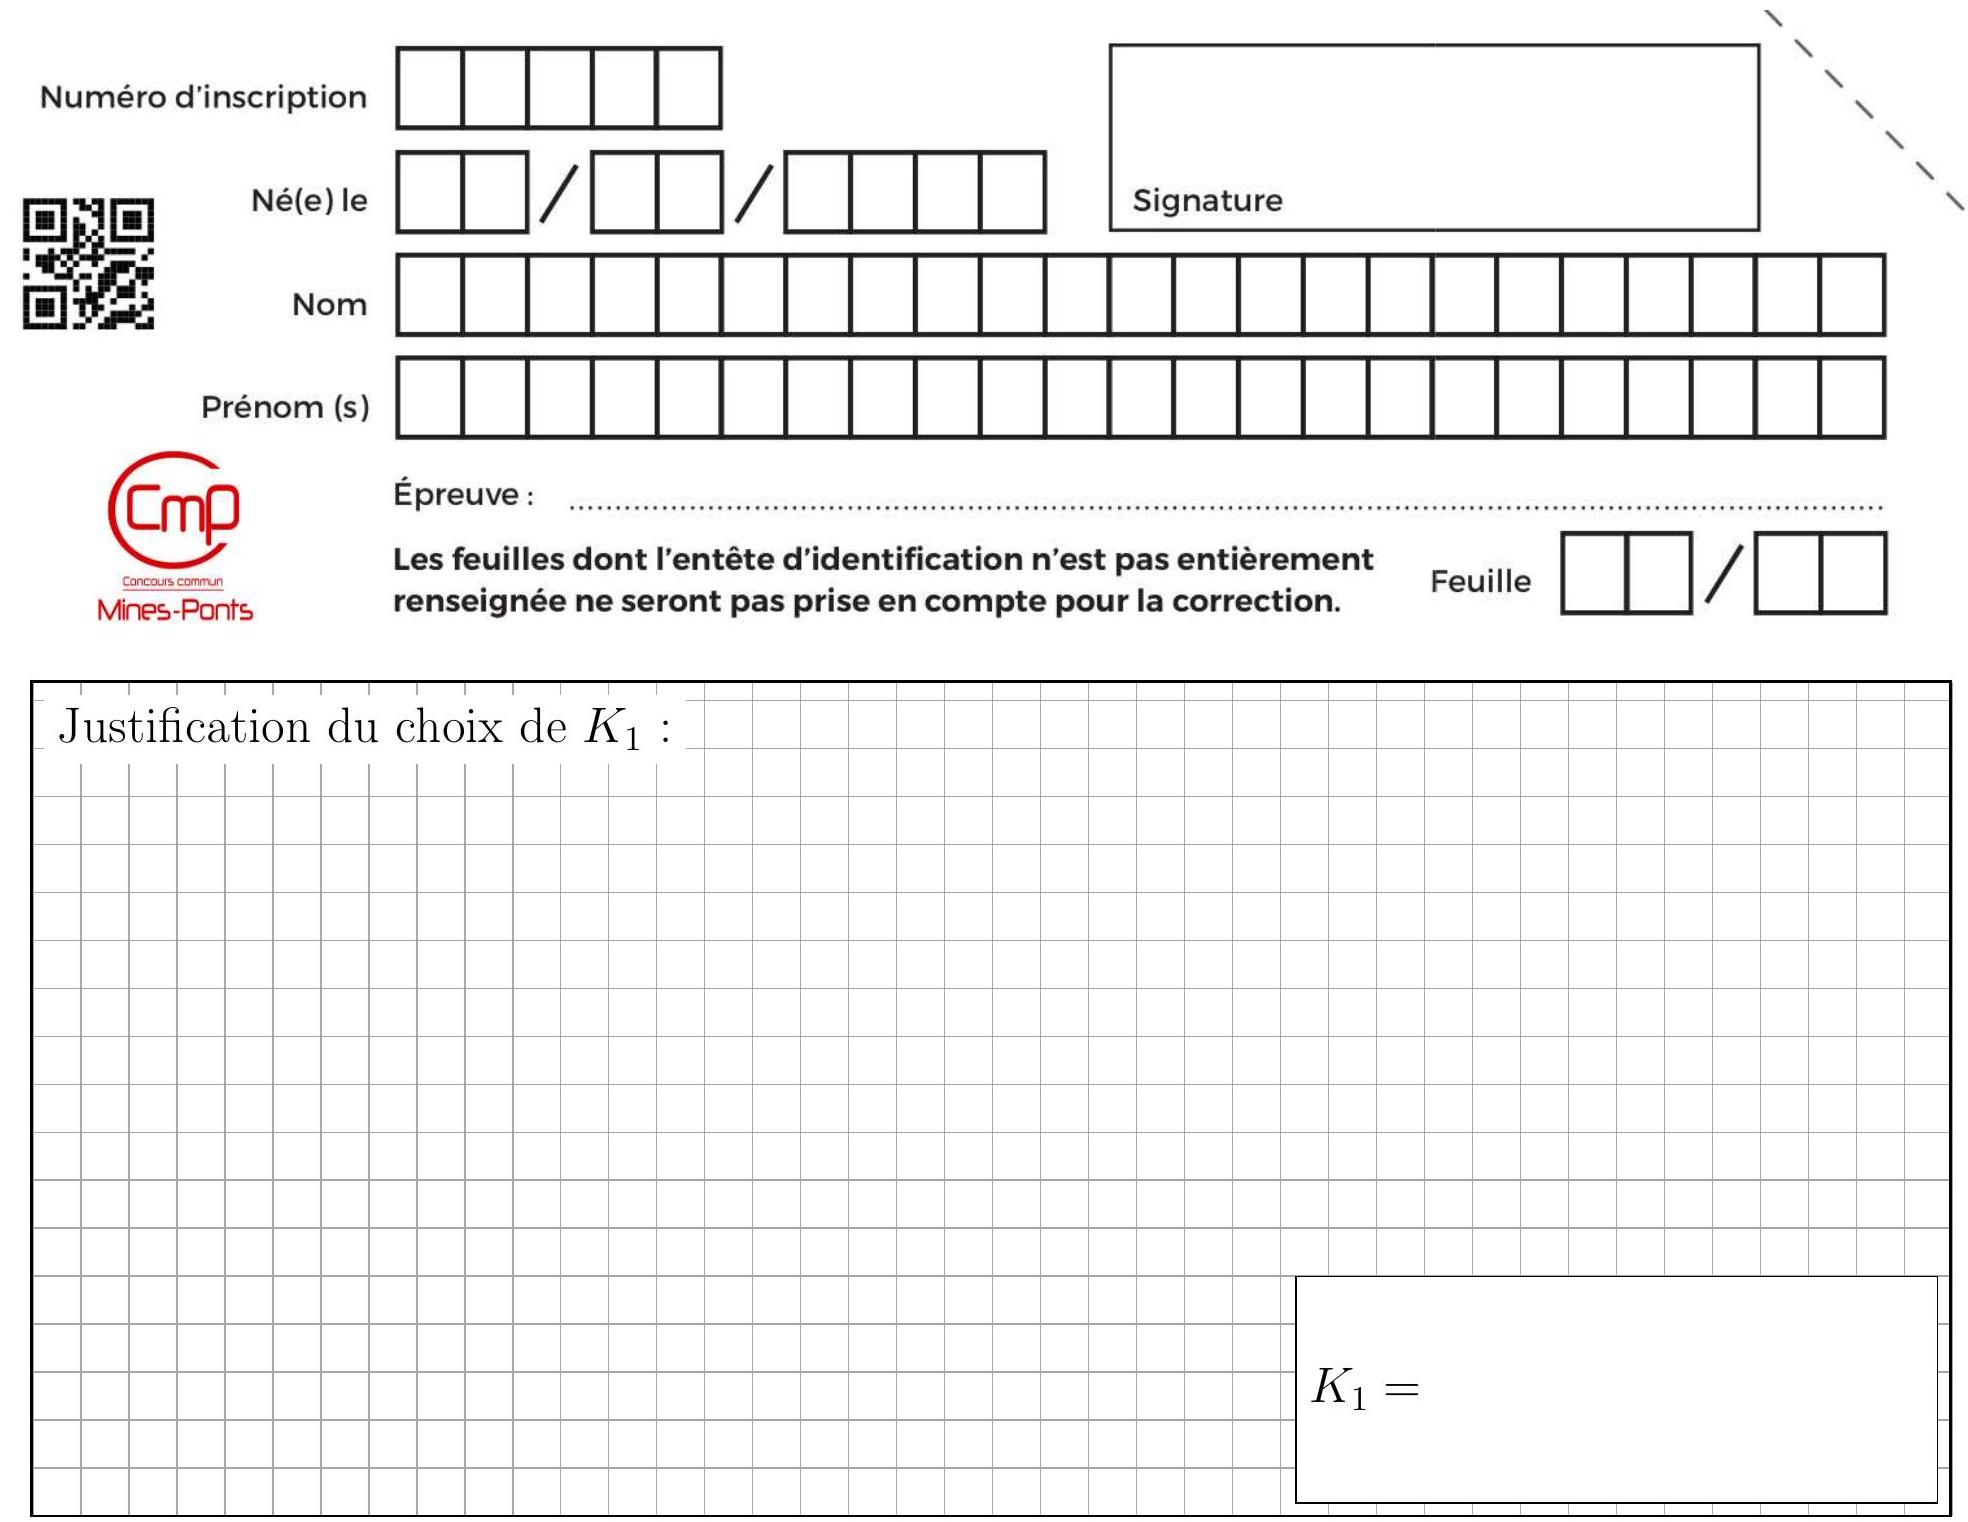
\includegraphics[max width=\textwidth]{2024_04_26_3285cfc264024262add0g-32}
\end{center}

Question 25

$\tau_{2}=$

$\tau_{3}=$

\begin{center}
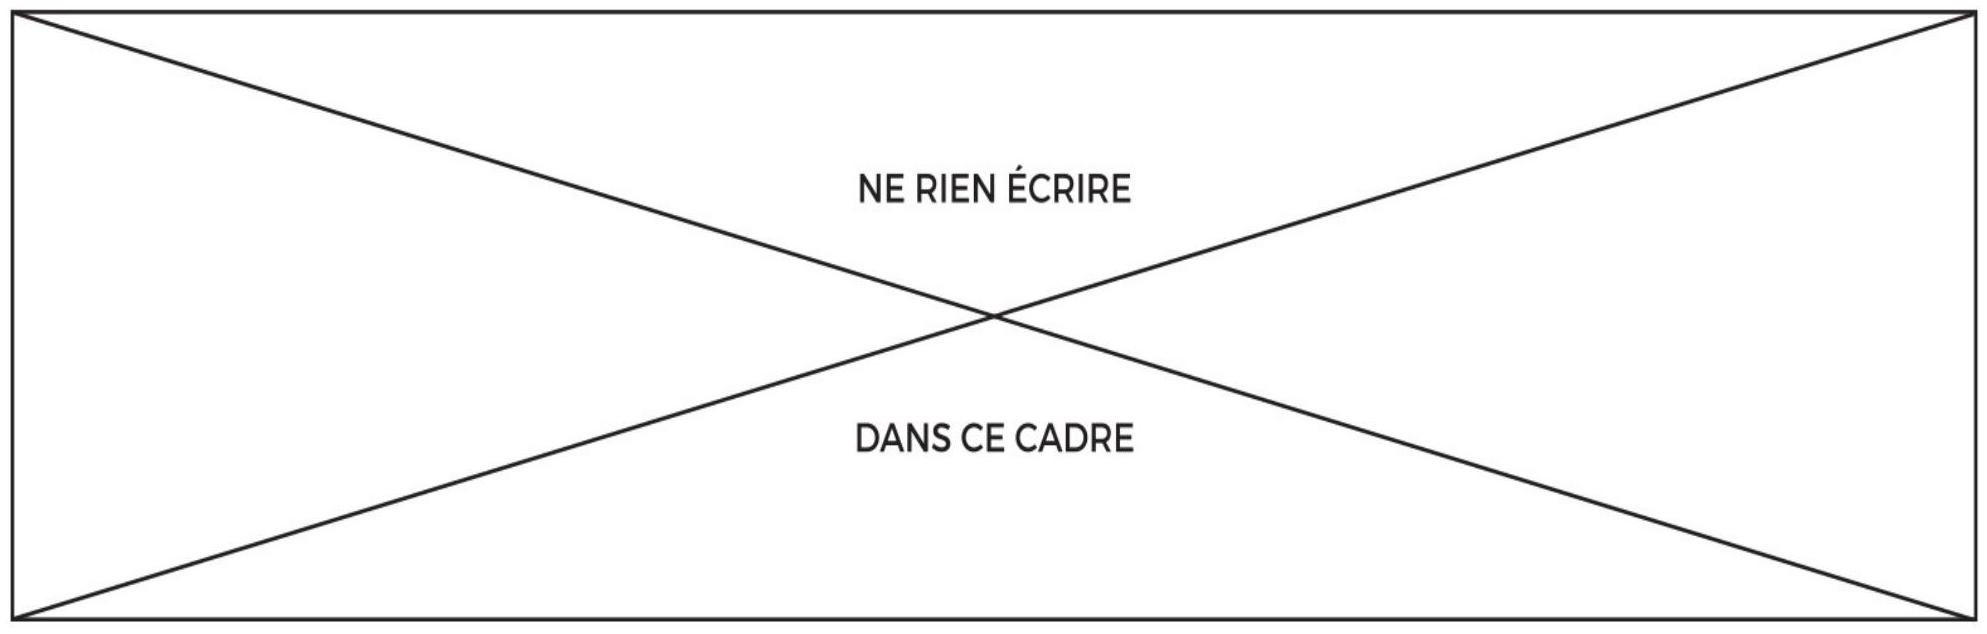
\includegraphics[max width=\textwidth]{2024_04_26_3285cfc264024262add0g-33}
\end{center}

Question 26 - Exigence 3.2:

Exigence 3.3 :

Question $27^{-}$Intérêt de la chaîne d'action BF :

Question 28

$$
H_{B O}(p)=
$$

Question 29\\
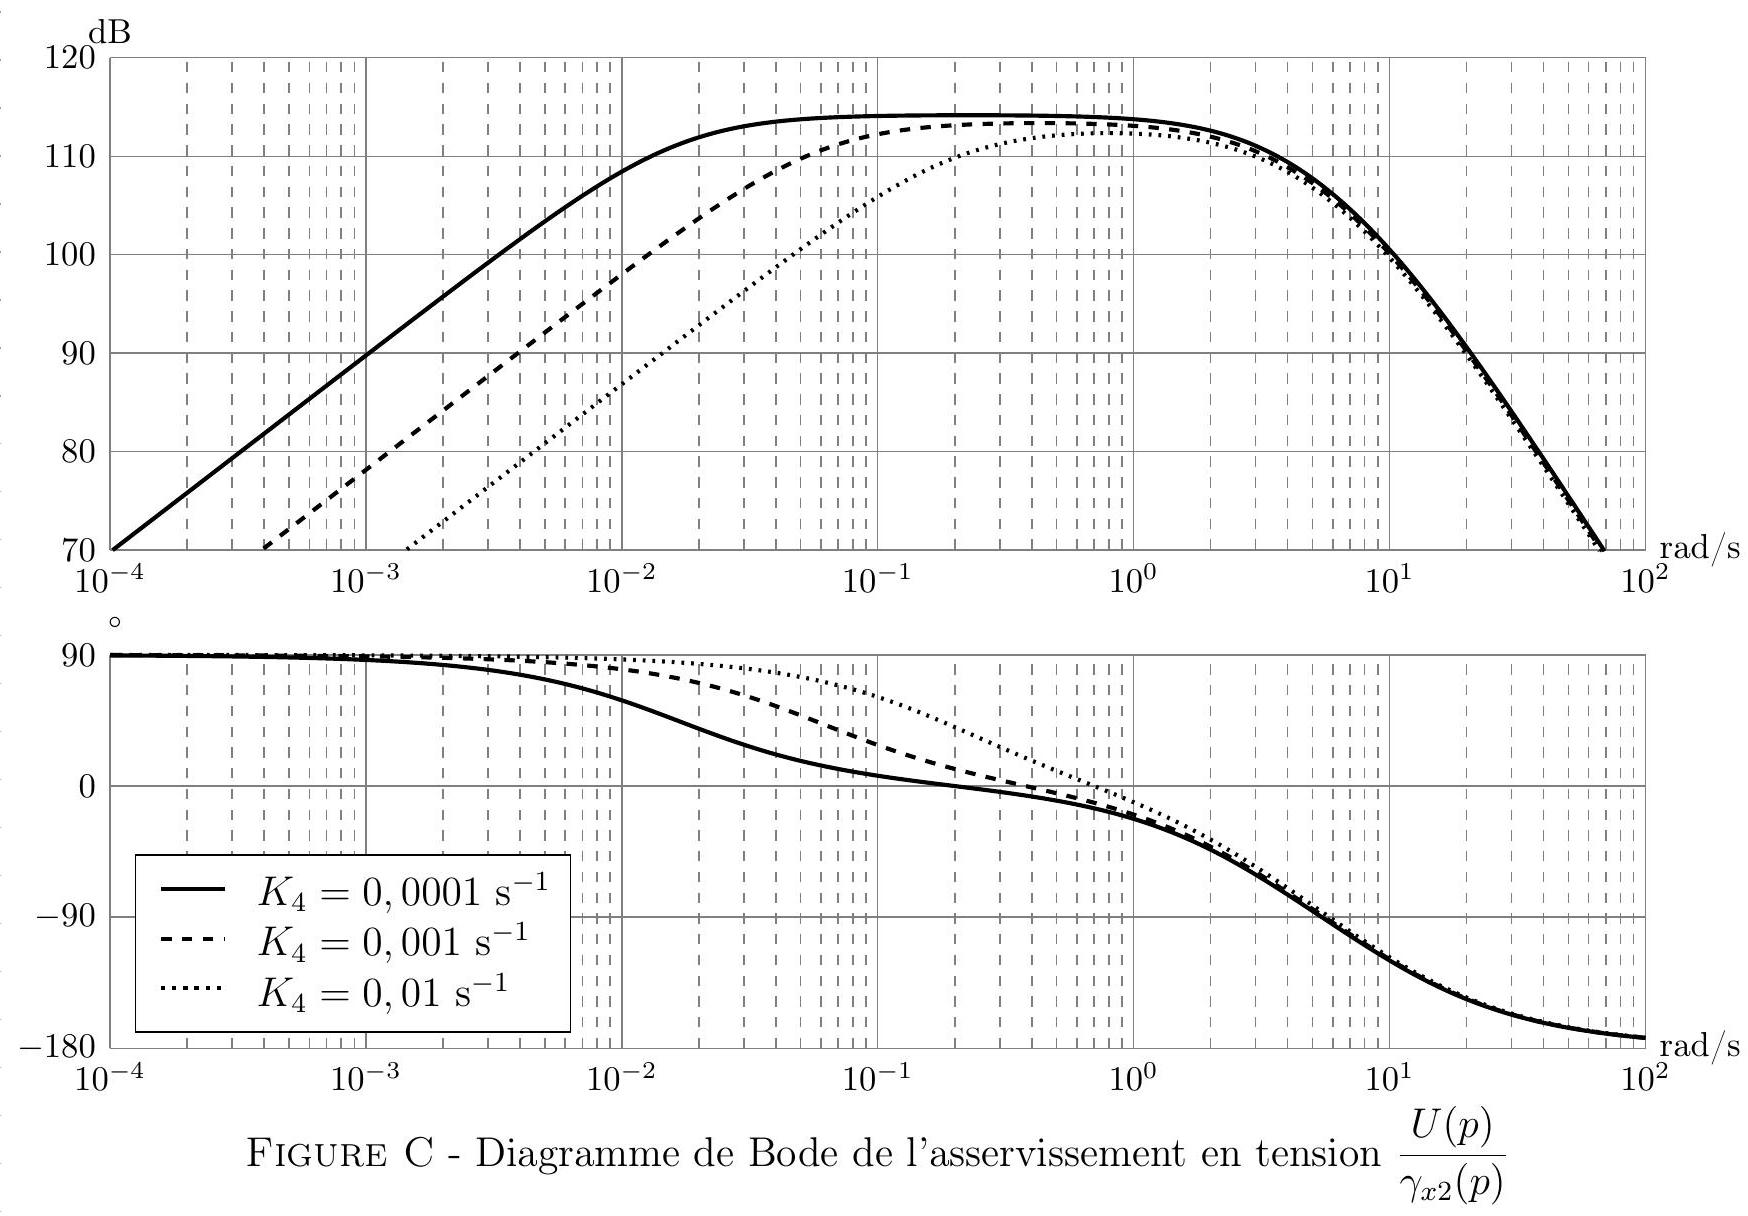
\includegraphics[max width=\textwidth, center]{2024_04_26_3285cfc264024262add0g-34}

$$
K_{4}=
$$

\section*{Question 30}

\end{document}